\documentclass[12pt]{article}
\usepackage[margin=0.5in]{geometry}
\usepackage{amsmath}
\usepackage{amsfonts}
\usepackage{amssymb}
\usepackage{enumitem}
\usepackage{graphicx}
\usepackage{tikz}
\usepackage{xcolor}
\usepackage{hyperref}


\title{Reinforcement Learning Notes}
\author{Generated from Lecture Notes for CSCI 6904 (Deep Reinforcement Learning)}
\date{\today}


\begin{document}

\maketitle
\tableofcontents

\newpage

\section{Formalization of the RL Problem }


\subsection{Markov Property}
\textbf{A state $S_t$ is Markov if $p(S_{t+1} \mid S_t) = p(S_{t+1} \mid S_1, \dots, S_t)$. This means the future is conditionally independent of the past, given the present state.} \\
Or \\
The Markov property, also known as the ``memoryless property", is a characteristic of stochastic processes where the future state of a system depends only on its current state, not on its past history.

\subsection{Markov Decision Process (MDP)}
An MDP is defined as a tuple $\langle \mathcal{S}, \mathcal{A}, P, R, \gamma \rangle$ where:
\begin{itemize}
    \item $\mathcal{S}$: The set of states.
    \item $\mathcal{A}$: The set of actions.
    \item $P$: The state-transition probability matrix, where $p(s'|s,a) = \Pr\{S_t = s' \mid S_{t-1} = s, A_{t-1} = a\}$.
    \item $R$: The reward function, where $r(s,a) = \mathbb{E}[R_t \mid S_{t-1} = s, A_{t-1} = a]$.
    \item $\gamma \in [0,1]$: The discount rate.
\end{itemize}
Goal: Find the optimal policy $\pi^*(a|s) = \arg\max_\pi \mathbb{E}_\pi [R_{t+1} + \gamma R_{t+2} + \gamma^2 R_{t+3} + \cdots \mid S_t = s]$.


\subsection{Goals and Rewards}
Rewards define the objective of the problem. A policy's goal is to maximize the expected cumulative discounted rewards over time.

\subsection{Discount Rate $\gamma$}
The discount rate $\gamma$ controls the preference for immediate versus future rewards. A value of $\gamma=0$ results in a myopic agent that only considers immediate rewards, while $\gamma=1$ makes the agent treat all future rewards equally, assuming the task eventually terminates.

\subsection{Returns and Episodes}
The return $G_t$ is the total discounted reward from time step $t$. It is defined as:
\begin{itemize}
    \item For continuing tasks: $G_t = \sum_{k=0}^\infty \gamma^k R_{t+k+1}$.
    \item For episodic tasks: $G_t = \sum_{k=0}^{T-t-1} \gamma^k R_{t+k+1}$, where $T$ is the terminal time step.
\end{itemize}
The return can be expressed recursively as $G_t = R_{t+1} + \gamma G_{t+1}$, with $G_T = 0$.

\subsection{Partially Observable MDP (POMDP)}
A POMDP is a generalization of an MDP defined as a tuple $\langle \mathcal{S}, \mathcal{A}, \mathcal{O}, P, R, E, \gamma \rangle$, which includes a set of observations $\mathcal{O}$ and an emission probability $E$, defined as $p(o_t \mid s_t)$. In a POMDP, the agent's policy is based on observations, $\pi(a|o)$, rather than states.


\section{Major Components of an RL Agent }

\subsection{Policy}
An agent's behavior maps states to actions.
\begin{itemize}
    \item Deterministic: $a = \pi(s)$.
    \item Stochastic: $\pi(a|s) = p(a|s)$.
\end{itemize}

\subsection{Value Function}
Prediction of expected return.
\begin{itemize}
    \item State-value: $v_\pi(s) = \mathbb{E}_\pi[G_t \mid S_t = s] = \mathbb{E}_\pi[\sum_{k=0}^\infty \gamma^k R_{t+k+1} \mid S_t = s]$.
    \item Action-value (Q-function): $q_\pi(s,a) = \mathbb{E}_\pi[G_t \mid S_t = s, A_t = a]$.

\end{itemize}
    If we represent  $V_\pi(s)$ in terms of Q value, then:

    $$
    V_\pi(s) = \sum_a \pi(a|s) Q_\pi(s,a) ]
    $$

\subsubsection*{Bellman Equation}

The Bellman equation relates a state's value to its immediate reward and the discounted value of the next state.

For a policy $\pi$ (state-value form):
$$
V_\pi(s) = \sum_a \pi(a|s) \sum_{s'} P(s'|s,a) [ R(s,a,s') + \gamma V_\pi(s') ]
$$



Meaning:
\begin{itemize}
    \item Weight actions by policy probability.
    \item Weight next states by transition probability.
    \item Add immediate reward + discounted future value.
\end{itemize}

\subsection{Optimal Value Function}
For optimal $V_*(s)$:
$$
V_*(s) = \max_a \sum_{s'} P(s'|s,a) [ R(s,a,s') + \gamma V_*(s') ]
$$
Replace sum over actions with max for best choice.

\subsection{Bellman Expectation Equation}
The Bellman expectation equation for the state-value function $V_\pi(s)$ is:
$$
V_\pi(s) = \mathbb{E}_\pi [ R_{t+1} + \gamma V_\pi(S_{t+1}) \mid S_t=s ]
$$
Here, the expectation operator $\mathbb{E}_\pi$ represents an average over actions selected by the policy $\pi$ and the subsequent next states produced by the environment's dynamics. It can be conceptually understood as answering the question: ``On average, if I follow policy $\pi$ from this state, what will I get?''


\subsection{Optimality in the Bellman Equation}
The relationship between prediction and control problems is central to Reinforcement Learning:
\begin{itemize}
    \item \textbf{Prediction problem:} Given a policy $\pi$, find its value function $V_\pi$.
    \item \textbf{Control problem:} Find the optimal policy $\pi_*$ that maximizes the return.
\end{itemize}

The Bellman optimality equation is what we solve to find the optimal value function $V_*$:
$$
V_*(s) = \max_a \mathbb{E} \big[ R_{t+1} + \gamma V_*(S_{t+1}) \mid S_t=s, A_t=a \big]
$$
Once we have the optimal value function $V_*$, the optimal policy $\pi_*$ can be found by acting greedily with respect to it:
$$
\pi_*(s) = \arg\max_a \sum_{s'} P(s'|s,a) \big[ R(s,a,s') + \gamma V_*(s') \big]
$$
\subsection{Recap}
\begin{itemize}
    \item Bellman expectation: value = average reward + average future value under $\pi$.
    \item Bellman optimality: value = best reward + best future value possible.
\end{itemize}


\subsection{Model}
An agent's representation of its environment.
\begin{itemize}
    \item Dynamics: $p(s',r|s,a) = \Pr\{S_{t+1}=s', R_{t+1}=r \mid S_t=s, A_t=a\}$.
    \item State transition: $p(s'|s,a)$.
    \item Reward: $r(s,a) = \mathbb{E}[R_{t+1} \mid S_t=s, A_t=a]$.
\end{itemize}

\subsection{Categorizing RL Agents}
\begin{itemize}
    \item \textbf{Policy-based}: A policy, but no value function.
    \item \textbf{Value-based}: A value function, with an implicit policy.
    \item \textbf{Actor-Critic}: Both a policy and a value function.
    \item \textbf{Model-free}: Learns policy or value function, but no model. Learns directly from experience without building model of the environment.
    \item \textbf{Model-based}: A policy or value function, plus a model. Learns the $p(s',r|s,a)$ (state transition probability and the reward) and uses it for planning.
\end{itemize}
\begin{tabular}{|p{0.15\linewidth}|p{0.15\linewidth}|p{0.2\linewidth}|p{0.2\linewidth}|p{0.2\linewidth}|}
\hline
\textbf{Category} & \textbf{Core Idea} & \textbf{How It Works} & \textbf{Pros} & \textbf{Cons} \\
\hline
\textbf{Policy-based} & Learn the policy directly (e.g., \textbf{REINFORCE, PPO}). & Use gradients to adjust policy parameters, often with randomness. & Handles continuous actions well; learns varied strategies. & Can be sample-inefficient and unstable. \\
\hline
\textbf{Value-based} & Learn a value function, pick best actions (e.g., \textbf{DQN, Double DQN}). & Update values (like Q-values) and act greedily. & Efficient for discrete tasks; stable targets. & Struggles with continuous actions; risk of overestimation. \\
\hline
\textbf{Actor-Critic} & Combine policy and value function (e.g., \textbf{A2C, SAC}). & Actor chooses actions, critic evaluates them. & Merges strengths of both; handles continuous actions well. & Coupled training can be unstable; needs careful tuning. \\
\hline
\textbf{Model-free} & Learn from direct experience only (e.g., \textbf{PPO, DQN}). & Learn policy/values via trial and error. & Simple and robust when modeling is hard. & Needs lots of data; no lookahead planning. \\
\hline
\textbf{Model-based} & Learn/use environment model (e.g., \textbf{Dyna-Q, Dreamer}). & Simulate future steps to improve. & Efficient; allows long-term planning. & Model errors can mislead; hard to learn accurate models. \\
\hline
\end{tabular}




\section{Introduction to Policy Gradient Methods }

Policy gradient method means it directly optimizes the policy by taking steps in the direction of the gradient of some objective function.

\subsection{Policy}
The parameterized policy is defined as: $\pi(a|s, \theta) = \Pr(A_t = a \mid S_t = s, \theta_t = \theta)$.

\begin{itemize}
    \item \textbf{Discrete Actions}: A softmax policy, where $\pi(a|s, \theta) = \frac{e^{h(s,a,\theta)}}{\sum_b e^{h(s,b,\theta)}}$, and $h(s,a,\theta)$ is a numerical preference for action $a$.
    \item \textbf{Continuous Actions}: A Gaussian policy, where the action is sampled from a normal distribution, $a \sim \mathcal{N}(\mu(s,\theta), \sigma^2(s,\theta))$. The probability density function is given by $\pi(a|s,\theta) = \frac{1}{\sigma_\theta(s) \sqrt{2\pi}} \exp\left( -\frac{(a - \mu_\theta(s))^2}{2\sigma_\theta^2(s)} \right)$.
\end{itemize}

\subsection{Objective}
The objective is to find the parameter $\theta$ that maximizes the expected return $J(\theta)$, which is defined as:
$$
J(\theta) \doteq \mathbb{E}_{\pi_\theta}[G_t \mid S_t = s_0] = v_{\pi_\theta}(s_0)
$$
Policy gradient methods achieve this by using an iterative update rule, often referred to as \textbf{Gradient Ascent}:
$$
\theta_{t+1} = \theta_t + \alpha \nabla_\theta J(\theta_t)
$$

\section{Policy Gradients for One-Step MDPs / Contextual Bandits}

One-step MDPs are defined as a process where an agent:
\begin{itemize}
    \item Starts in a state $s$ sampled from a distribution $d(s)$.
    \item Takes an action $a$ sampled from the policy $\pi_\theta(a|s)$.
    \item Receives a reward $r = R_{s,a}$ and the episode terminates.
\end{itemize}

\subsubsection*{Example: An online ad system} \\

\begin{itemize}
    \item States = user contexts: \{sports-fan, tech-enthusiast, foodie\}.
    \item The platform sees users with frequencies: $d(\text{sports}) = 0.5$, $d(\text{tech}) = 0.3$, $d(\text{foodie}) = 0.2$ (this is $d(s)$).
    \item Each time a user arrives:
    \begin{itemize}
        \item The system observes $s$ sampled from $d(s)$.
        \item Chooses an ad (action).
        \item Gets a click/no-click reward.
        \item The interaction ends.
    \end{itemize}
\end{itemize}



The objective is to maximize the expected reward, given by:
$$
J(\theta) = \mathbb{E}_{\pi_\theta}[r] = \sum_s d(s) \sum_a \pi_\theta(a|s) R_{s,a}
$$
The policy gradient is then calculated as:
$$
\nabla_\theta J(\theta) = \mathbb{E}_{\pi_\theta} [ \nabla_\theta \log \pi_\theta(a|s) \cdot r ] \approx \frac{1}{N} \sum_i \nabla_\theta \log \pi_\theta(A_i|S_i) \cdot R_{S_i,A_i}
$$
The policy parameters are updated using a gradient ascent rule:
$$
\theta \leftarrow \theta + \alpha \nabla_\theta J(\theta)
$$
This approach differs from Supervised Learning (SL) Maximum Likelihood in that the RL update is weighted by the reward $r$, whereas the SL update is an unweighted average.

\subsection{Algorithm ($\sim$ REINFORCE for one-step)}
\begin{enumerate}
    \item Run the policy: Sample a state $s \sim d(s)$ and an action $a \sim \pi_\theta(a|s)$.
    \item Compute the gradient estimate: $\nabla_\theta J(\theta) = \frac{1}{N} \sum_i \nabla_\theta \log \pi_\theta(A_i|S_i) R_{S_i,A_i}$.
    \item Update the policy parameters: $\theta \leftarrow \theta + \alpha \nabla_\theta J(\theta)$.
\end{enumerate}
\section{Policy Gradients for Multi-Step MDPs }

\subsection{Objective}
The objective is to maximize the expected return from a starting state, which is equivalent to the state-value function:
$$ J(\theta) = \mathbb{E}_{\pi_\theta}[G_t \mid S_t = s_0] = v_{\pi_\theta}(s_0) $$

\subsection{Policy Gradient Theorem}
The policy gradient theorem provides a way to compute the gradient of the objective function:
$$ \nabla_\theta J(\theta) \propto \mathbb{E}_{\pi_\theta} \left[ \nabla_\theta \log \pi_\theta(a|s) \cdot q_\pi(s,a) \right] $$
This is often approximated with the Monte Carlo return $G_t$:
$$ \nabla_\theta J(\theta) \approx \mathbb{E}_{\pi_\theta} \left[ \nabla_\theta \log \pi_\theta(a|s) \cdot G_t \right] $$
This replaces the instantaneous reward with a long-term value $q_\pi(s,a)$ to guide learning.

\subsection{REINFORCE Algorithm}
\begin{enumerate}
    \item Sample trajectories $\{\tau_i\}$ from the policy $\pi_\theta$.
    \item For each time step $t$ in a trajectory, compute the return $G_t^i = \sum_{k=t+1}^{T} \gamma^{k-t-1} R_k^i$.
    \item Estimate the policy gradient:
    $$ \nabla_\theta J(\theta) \approx \frac{1}{N} \sum_{i=1}^N \sum_{t=1}^{T_i} \nabla_\theta \log \pi_\theta(A_t^i | S_t^i) G_t^i $$
    \item Update the policy parameters: $\theta \leftarrow \theta + \alpha \nabla_\theta J(\theta)$.
\end{enumerate}
\textbf{Note}: This algorithm encourages good trajectories by increasing the probability of actions that lead to high returns.
\begin{itemize}
    \item \textbf{Discrete actions}: Use a softmax policy.
    \item \textbf{Continuous actions}: Use a Gaussian policy.
\end{itemize}
This method suffers from high variance in gradient estimates.

\subsection{REINFORCE with Baseline}
A baseline $b(s)$ (e.g., the state-value function $v(s)$) can be subtracted from the return to reduce variance without changing the expected value of the gradient.
$$ \nabla_\theta J(\theta) \propto \mathbb{E}_{\pi_\theta} \left[ \nabla_\theta \log \pi_\theta(a|s) \cdot (q_\pi(s,a) - b(s)) \right] $$

\subsubsection{Algorithm}
\begin{enumerate}
    \item Sample trajectories $\{\tau_i\}$ from $\pi_\theta$.
    \item Compute returns $G_t^i$.
    \item Estimate the policy gradient using a learned state-value function $\hat{v}_w(s)$ as the baseline:
    $$ \nabla_\theta J(\theta) \approx \frac{1}{N} \sum_{i=1}^N \sum_{t=1}^{T_i} \nabla_\theta \log \pi_\theta(A_t^i | S_t^i) (G_t^i - \hat{v}_w(S_t^i)) $$
    \item Update the policy parameters: $\theta \leftarrow \theta + \alpha_\theta \nabla_\theta J(\theta)$.
    \item Define the value function loss:
    $$ L(w) = \frac{1}{N} \sum_{i=1}^N \sum_{t=1}^{T_i} (G_t^i - \hat{v}_w(S_t^i))^2 $$
    \item Update the value function parameters: $w \leftarrow w - \alpha_w \nabla_w L(w)$.
\end{enumerate}

\section{Off-Policy Policy Gradients }

\subsection{Concepts}
\begin{itemize}
    \item \textbf{On-policy} methods learn a policy from experience collected by that same policy.
    \item \textbf{Off-policy} methods learn a target policy $\pi$ using data generated by a different behavior policy $\mu$.
\end{itemize}
Off-policy learning offers key advantages: it can reuse old data, allows the agent to learn an optimal policy while actively exploring with a different behavior policy, and enables learning about multiple policies simultaneously.

\subsection{Importance Sampling}
Importance sampling is a technique that allows us to estimate the expected value of a function under one distribution, using samples from another. This is the core of off-policy policy gradients.
$$ \mathbb{E}_{x \sim p}[f(x)] = \mathbb{E}_{x \sim q} \left[ f(x) \frac{p(x)}{q(x)} \right] $$
The term $\frac{p(x)}{q(x)}$ is the importance sampling weight, which corrects for the difference between the two distributions.

\subsection{Off-Policy REINFORCE with Importance Sampling}
This method adapts REINFORCE to an off-policy setting by using importance sampling. It allows the algorithm to learn from data collected by an older policy, $\pi_{\theta_{old}}$.
The gradient is estimated using the importance sampling weight to correct for the change in policy:
$$ \nabla_\theta J(\theta) \approx \frac{1}{N} \sum_{i=1}^N \sum_{t=1}^{T_i} \frac{\pi_\theta(A_t^i | S_t^i)}{\pi_{\theta_{old}}(A_t^i | S_t^i)} \nabla_\theta \log \pi_\theta(A_t^i | S_t^i) G_t^i $$
The parameters are then updated:
$$ \theta \leftarrow \theta + \alpha \nabla_\theta J(\theta) $$
After the update, the old policy is replaced by the new one:
$$ \theta_{old} \leftarrow \theta $$
This approach is notably used in algorithms like Proximal Policy Optimization (PPO), which is essential for training large language models like those in ChatGPT. PPO clips the importance sampling weight to prevent excessively large updates, which helps stabilize learning.

\section{Case Study: Dialog Systems like ChatGPT }

\subsection{Training Phases}
The development of advanced dialog systems like ChatGPT typically follows three key phases:
\begin{enumerate}
    \item \textbf{Pretraining (LM)}: A large language model (LM) is first pretrained on a vast corpus of text to learn language patterns and predict the next token.
    \item \textbf{Instruction Finetuning (SL)}: The pretrained model is then finetuned on a dataset of high-quality instructions and responses using supervised learning (SL) to better follow directions.
    \item \textbf{Reinforcement Learning with Human Feedback (RLHF)}: The model is further aligned with human preferences using reinforcement learning.
\end{enumerate}

\subsection{Reinforcement Learning with Human Feedback (RLHF)}
RLHF leverages policy gradients to refine the model's behavior based on human input. The process involves:
\begin{enumerate}
    \item \textbf{Response Sampling}: The policy $\pi_\theta$ generates a response (action $a$) to a given prompt (state $s$).
    \item \textbf{Human Feedback}: Human labelers provide feedback on the responses, often by ranking them.
    \item \textbf{Reward Model Training}: A separate reward model, $r_\psi(s,a)$, is trained to predict the human preference score for any response, learning from the collected rankings.
    \item \textbf{Policy Update}: The policy is updated using a policy gradient algorithm with the reward signal from the reward model. A simplified update rule is:
    $$ \nabla_\theta J(\theta) \approx \frac{1}{N} \sum_{i=1}^N \nabla_\theta \log \pi_\theta(A_i | S_i) r(S_i, A_i) $$

    \item \textbf{Over Optimization in Dialog systems:}
    $J(\theta) = \mathbb{E}_{\pi_{\theta}}[r] - \beta D_{KL}(\pi_{\theta}||\pi_{\beta})$
    
    \item \textbf{Off-Policy Considerations}: To improve sample efficiency, off-policy methods with importance sampling are used. A \textbf{KL-divergence penalty} is also added to the loss function to prevent the new policy from deviating too drastically from the reference policy, thus maintaining model stability and preventing reward hacking.
\end{enumerate}

\section{Actor-Critic Methods }

\subsection{Recap: Policy Gradient Methods}

\subsubsection{Monte-Carlo Policy Gradient (REINFORCE)}
\begin{itemize}
    \item \textbf{Objective}: The goal is to maximize the expected return from a starting state, represented by the state-value function:
    $$ J(\theta) = \mathbb{E}_{\pi_\theta}[G_t \mid S_t = s_0] = v_{\pi_\theta}(s_0) $$
    \item \textbf{Policy Gradient Theorem}: The gradient is estimated as the expectation of the log-policy gradient scaled by the action-value function:
    $$ \nabla_\theta J(\theta) \propto \mathbb{E}_{\pi_\theta} [\nabla_\theta \log \pi_\theta(a|s) q_\pi(s,a)] $$
    \item \textbf{Update Rule}: The parameters are updated in the direction of the sampled return $G_t$, which is a Monte-Carlo estimate of $q_\pi(s,a)$:
    $$ \theta_{t+1} = \theta_t + \alpha \nabla_\theta \log \pi_\theta(A_t|S_t) G_t $$
\end{itemize}
This method estimates the action-value function using a complete trajectory's return, which, while unbiased, can have high variance.

\subsubsection{REINFORCE with Baseline}
To address the high variance of REINFORCE, a baseline $b(s)$ is introduced.
\begin{itemize}
    \item \textbf{Modified Gradient}: The gradient is now proportional to the advantage function, which is the difference between the action-value and a state-dependent baseline. This reduces variance without changing the expected value of the gradient.
    $$ \nabla_\theta J(\theta) \propto \mathbb{E}_{\pi_\theta} [\nabla_\theta \log \pi_\theta(a|s) (q_\pi(s,a) - b(s))] $$
    \item \textbf{Update Rule}: The update is based on the advantage estimate:
    $$ \theta_{t+1} = \theta_t + \alpha \nabla_\theta \log \pi_\theta(A_t|S_t) (G_t - b(S_t)) $$
    \item A common and effective baseline is a learned value function, $b(S_t) = \hat{v}(S_t, w)$.
\end{itemize}

\subsection{Actor-Critic Methods}

\subsubsection{Core Concepts}
Actor-Critic methods combine a policy network (the \textbf{actor}) with a value function network (the \textbf{critic}).
\begin{itemize}
    \item The \textbf{actor} is the policy, parameterized by $\theta$, which chooses the action.
    \item The \textbf{critic} is a value function, parameterized by $w$, which estimates the value of the state or state-action pair.
    \item Instead of waiting for a full trajectory's return (Monte Carlo), the actor-critic method uses the critic's value estimate to update the actor. This allows for updates at every step, reducing the variance and speeding up learning.
\end{itemize}
The critic is used to bootstrap, providing a value estimate to guide the actor.

\subsubsection{Advantage Actor-Critic}
This approach uses the \textbf{advantage function} as the critic's signal to the actor. \textbf{The advantage function, $A^{\pi}(s,a)$, measures how much better a specific action $a$ is compared to the expected value of the state, $V^{\pi}(s)$.}
\begin{itemize}
    \item \textbf{Advantage function}:
    $A^\pi(s,a) = Q^\pi(s,a) - V^\pi(s)$ \\
    
     or using the Bellman equation:
    $A^\pi(s,a) = r + \gamma V^\pi(s') - V^\pi(s)$
    \item \textbf{Advantage estimate}: A common way to estimate the advantage is with the Temporal-Difference (TD) error:
    $$ \hat{A}(S_t, A_t) = R_{t+1} + \gamma \hat{v}_w(S_{t+1}) - \hat{v}_w(S_t) $$
    This is an estimate of how much the reward was better (or worse) than expected.
    \item \textbf{Gradient Update}: The policy gradient is then estimated using this advantage signal:
    $$ \nabla_\theta J(\theta) \approx \nabla_\theta \log \pi_\theta(A_t|S_t) \hat{A}(S_t, A_t) $$
\end{itemize}

\subsubsection{ (Batch) Advantage Actor-Critic Algorithm}
This algorithm trains both the actor and the critic networks simultaneously using a batch of sampled trajectories.
\begin{enumerate}
    \item \textbf{Sample Trajectories}: Collect a set of trajectories $\{\tau_i\}$ using the current policy $\pi_\theta$.
    \item \textbf{Update Critic}: The critic network's parameters $w$ are updated to minimize the squared TD-error loss.
    $$ L(w) = \frac{1}{N} \sum_{i=1}^N \sum_{t=1}^{T_i} (R_{t+1}^i + \gamma \hat{v}_w(S_{t+1}^i) - \hat{v}_w(S_t^i))^2 $$
    The parameters are updated via gradient descent: $w \leftarrow w - \alpha_w \nabla_w L(w)$.
    \item \textbf{Evaluate Advantage}: For each step in the batch, the advantage estimate is calculated using the updated critic.
    $$ \hat{A}(S_t^i, A_t^i) = R_{t+1}^i + \gamma \hat{v}_w(S_{t+1}^i) - \hat{v}_w(S_t^i) $$
    \item \textbf{Update Actor}: The actor network's parameters $\theta$ are updated using the batch of advantage estimates.
    $$ \nabla_\theta J(\theta) \approx \frac{1}{N} \sum_{i=1}^N \sum_{t=1}^{T_i} \nabla_\theta \log \pi_\theta(A_t^i | S_t^i) \hat{A}(S_t^i, A_t^i) $$
    The parameters are updated via gradient ascent: $\theta \leftarrow \theta + \alpha_\theta \nabla_\theta J(\theta)$.
\end{enumerate}

\subsubsection{Network Designs}
\begin{itemize}
    \item \textbf{Two-Network Design}: The actor and critic are two separate neural networks with their own parameters.
    \item \textbf{Shared-Network Design}: A single network is used, with a shared trunk that processes the state input, and two separate heads for outputting the policy (actor) and the value estimate (critic). This can be more parameter-efficient. \\

    A shared network design is considered parameter efficient because it uses each parameter (a weight in the model) for many different parts of the task.

This approach reduces the total number of parameters required. This, in turn, leads to several benefits for the model, including:
\begin{itemize}
\item Faster processing
\item Less memory usage
\item Better generalization to new tasks
\end{itemize}
This idea is a core principle in modern deep learning and multi-task learning systems.
\end{itemize}

\section{Dynamic Programming (DP) }

\subsection{Bellman Equations}
\begin{itemize}
    \item State-value: $v_\pi(s) = \sum_a \pi(a|s) \sum_{s',r} p(s',r|s,a) [r + \gamma v_\pi(s')]$.
    \item Action-value: $q_\pi(s,a) = \sum_{s',r} p(s',r|s,a) [r + \gamma \sum_{a'} \pi(a'|s') q_\pi(s',a')]$.
    \item Optimal state-value: $v^*(s) = \max_a \sum_{s',r} p(s',r|s,a) [r + \gamma v^*(s')]$.
    \item Optimal action-value: $q^*(s,a) = \sum_{s',r} p(s',r|s,a) [r + \gamma \max_{a'} q^*(s',a')]$.
\end{itemize}

\subsection{Iterative Policy Evaluation (Prediction)}
``If I follow this strategy, how good is each situation I'll encounter?'' This process does not alter the policy; it simply evaluates it. The algorithm estimates the ``value'' (long-term expected reward) of each state under a fixed policy $\pi$.\\

\textbf{Why is this useful?} You need to know if a policy is good before improving it. This is the ``prediction" part of RL.\\

\textbf{Input:} An MDP $\langle \mathcal{S}, \mathcal{A}, P, R, \gamma \rangle$ and a policy $\pi$.

\textbf{Output:} $v_\pi$.
\begin{enumerate}
    \item Start with an initial guess. Initialize $v_0(s) = 0$ for all $s \in \mathcal{S}$.
    \item Repeat until convergence:
    $v_{k+1}(s) = \sum_a \pi(a|s) \sum_{s',r} p(s',r|s,a) [r + \gamma v_k(s')]$ (Bellman equation).
    \item Stop when values stop changing much
\end{enumerate}

\subsection{Policy Iteration (Control)} 
This algorithm finds an optimal policy $\pi^*$ (the best actions to take in each state) and its corresponding optimal value function $V^*$. \\

\textit{PolicyIteration = Policy Evaluation + Policy Improvement}  (This is done iteratively)\\

It operates by alternating between evaluating the current policy and improving it, a process known as policy iteration.\\

\textbf{Why it is useful:}
Policy iteration is a control method, not just a prediction one. Its goal is to find the best possible strategy to maximize long-term rewards, making it a foundational algorithm for solving control problems in reinforcement learning.\\ \\
\textbf{Input:} MDP $\langle \mathcal{S}, \mathcal{A}, P, R, \gamma \rangle$.\\

\textbf{Output:} $v^*$, $\pi^*$. 
\begin{enumerate}
    \item Initialize $\pi_0$ arbitrarily (e.g., random actions).
    \item Policy Evaluation: Compute $v_{\pi_k}$ using iterative evaluation (section 9.2).
    \item Policy Improvement: $\pi_{k+1}(s) = \arg\max_a q_{\pi_k}(s,a) = \arg\max_a \sum_{s',r} p(s',r|s,a) [r + \gamma v_{\pi_k}(s')]$ (greedy choice based on current v).
    \item Repeat until $\pi_{k+1} = \pi_k$.
\end{enumerate}

\subsection{Value Iteration (Control)}
Similar to Policy Iteration, this algorithm finds an optimal policy $\pi^*$ and its value function $V^*$. It combines the evaluation and improvement steps into one by repeatedly applying the Bellman optimality equation to directly compute the optimal value function $V^*$, from which the optimal policy can be extracted.\\

\textbf{Why it is useful}
Value Iteration is a control method: it not only predicts but also finds the best strategy. It is simpler and often converges faster than Policy Iteration for large problems because it does not require a separate, exhaustive policy evaluation phase -- because it combines policy improvement and evaluation into a single update.\\ 

\begin{enumerate}
    \item Initialize $v_0(s) = 0$.
    \item Repeat until convergence:
    $v_{k+1}(s) = \max_a \sum_{s',r} p(s',r|s,a) [r + \gamma v_k(s')]$.
    \item Once converged, get Optimal policy: $\pi^*(s) = \arg\max_a \sum_{s',r} p(s',r|s,a) [r + \gamma v^*(s')]$.
\end{enumerate}

\section{Asynchronous Dynamic Programming}

Asynchronous value iteration is a method for finding the best policy in a Markov Decision Process (MDP) by updating the value of states one at a time, or in small groups, without waiting for a full sweep of all states. This contrasts with traditional, synchronous methods that update all states simultaneously. This flexibility often leads to faster convergence, especially for large state spaces.

\subsection*{How It Works}
Imagine a problem of finding the shortest path on a map with many cities (states).

\textbf{Synchronous Value Iteration} would be like a team of people simultaneously calculating the shortest distance from every single city to a destination. They all work on their assigned city at the same time and then, after everyone has finished, they collectively share and update their findings. If the map has a million cities, this is inefficient because the entire team must wait for the slowest person to finish their calculation before the next round of updates can begin.

\textbf{Asynchronous Value Iteration} is like having the same team work independently. One person calculates the distance for City A, another for City B, and so on. As soon as one person finds a new, better route for their city, they immediately update that city's value. This new information is instantly available for everyone else to use in their ongoing calculations. This continuous and immediate sharing of information allows the process to converge more quickly because no one is idle, waiting for the entire set of calculations to complete.

\subsection{Synchronous Dynamic Programming}
\begin{itemize}
    \item All states are \textbf{updated in parallel} at each iteration.
    \item Example: \textbf{Value Iteration}.
    \item For all $s \in S$:
        $$
        v_{k+1}(s) = \max_{a} \sum_{s',r} p(s',r|s,a)\big[r + \gamma v_k(s')\big]
        $$
    \item Each $v_{k+1}(s)$ update uses the previous $v_k(s')$ values.
\end{itemize}

\subsection{Asynchronous Dynamic Programming}
\begin{itemize}
    \item States can be \textbf{updated in any order}, possibly one at a time.
    \item Does not require full-sweep of all states per iteration.
    \item \textbf{Converges} as long as all states continue to be selected for updates.
\end{itemize}

\subsubsection{In-Place Dynamic Programming}
\begin{itemize}
    \item Use the latest available values for $v(s)$ during updates, not just those from previous iteration.
    \item For all $s \in S$:
        $$
        v(s) \leftarrow \max_{a} \sum_{s',r} p(s',r|s,a)[r + \gamma v(s')]
        $$
\end{itemize}

\subsubsection{Prioritized Sweeping}
\begin{itemize}
    \item Prioritize updates for states with largest Bellman error.
    \item Leads to faster convergence by focusing computation on relevant parts of the state space.
\end{itemize}

\subsubsection{Real-Time Dynamic Programming}
\begin{itemize}
    \item Updates guided by agent's actual experience.
    \item Utilizes the environment's feedback to steer which states are updated.
    \item Helps agent focus learning on states most relevant to its current task.
\end{itemize}

% Sample pseudocode for Asynchronous DP
\subsubsection*{Pseudocode: Asynchronous Value Iteration}
\begin{verbatim}
for iteration k = 1..K:
    for each selected state s (order may vary):
\end{verbatim}
\quad v(s) ← $max_a Σ_{s', r} p(s', r | s, a) [r + γ v(s')]$


\section{Model-Free Prediction }

\subsection{Monte-Carlo (MC) Learning}
\begin{itemize}
    \item Learn $v_\pi(s) = \mathbb{E}_\pi[G_t \mid S_t = s]$.
    \item MC Update: $V(s) \leftarrow V(s) + \alpha (G_t - V(s))$.
    \item Incremental: $N(s) \leftarrow N(s) + 1$; Where \textit{N(s)} is the total number of visits to state s so far (i.e., a state-visitation count)\\ 
    $V(s) \leftarrow V(s) + \frac{1}{N(s)}(G_t - V(s))$.
\end{itemize}

\subsection{Temporal-Difference (TD(0)) Learning}
\begin{itemize}
    \item Update: $V(S_t) \leftarrow V(S_t) + \alpha (R_{t+1} + \gamma V(S_{t+1}) - V(S_t)$.\\
    Where :
    $$TD.error = R_{t+1} + \gamma V(S_{t+1}) - V(S_t)$$
    $$Target = (R_{t+1} + \gamma V(S_{t+1})$$
    \item TD error: $\delta_t = R_{t+1} + \gamma V(S_{t+1}) - V(S_t)$.
\end{itemize}

\subsection{n-Step TD Learning}
\begin{itemize}
    \item n-step return: $G_{t:t+n} = R_{t+1} + \gamma R_{t+2} + \cdots + \gamma^{n-1} R_{t+n} + \gamma^n V(S_{t+n})$.
    \item Update: $V(S_t) \leftarrow V(S_t) + \alpha (G_{t:t+n} - V(S_t))$.
\end{itemize}

\section{Unified View}

\begin{figure}[htbp]
    \centering
    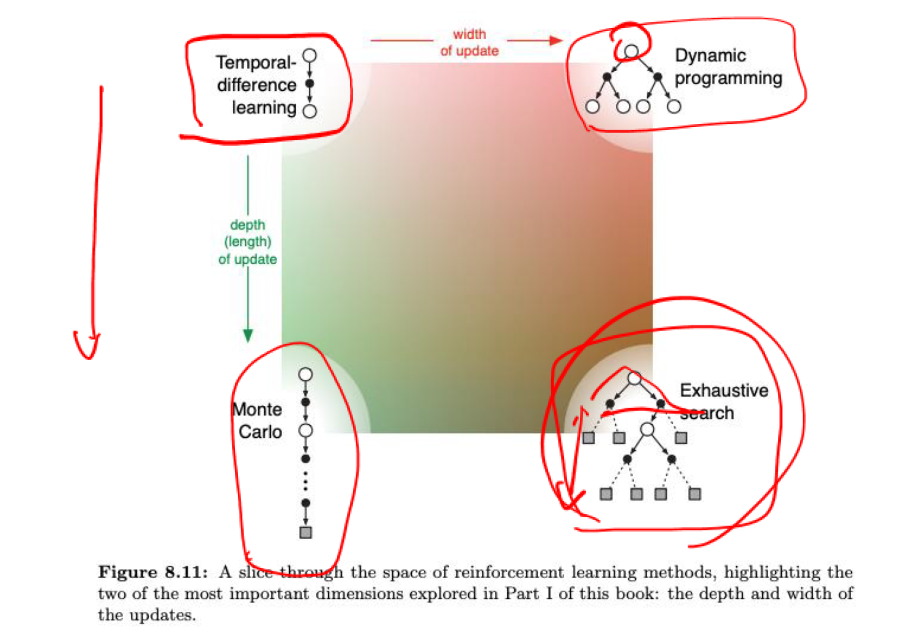
\includegraphics[width=0.5\linewidth]{images/unified_view.png}
    \caption{Unified View}
    \label{fig:placeholder}
\end{figure}

\textbf{What do ``depth" and ``width" mean?}

\textbf{Depth (length of update):}
Refers to how far into the future each update looks.
\begin{itemize}
    \item \textbf{Short depth:} Update uses immediate next state (e.g., TD learning).
    \item \textbf{Long depth:} Update could use entire episode or tree (e.g., Monte Carlo, exhaustive search).
\end{itemize}

\textbf{Width (branching in update):}
How many alternative actions or transitions are considered in each update.
\begin{itemize}
    \item \textbf{Narrow width:} Single trajectory or outcome (e.g., real experience).
    \item \textbf{Wide width:} All possible actions/states (e.g., dynamic programming, exhaustive search).
\end{itemize}

\section{TD($\lambda$): Simple Example with $\lambda=1/2$}

\subsection{Idea}
\begin{itemize}
    \item TD($\lambda$) averages several $n$-step returns, with weights $\lambda^{n-1}$.
    \item When $\lambda=0$: Only uses 1-step TD (TD(0)).
    \item When $\lambda=1$: Uses full return (Monte Carlo).
    \item At $\lambda = \frac{1}{2}$: Each longer return is included but weighted less. 
The 1-step return gets weight $1/2^{0} = 1$, the 2-step return gets weight $1/2^{1} = 0.5$, 
the 3-step return gets weight $1/2^{2} = 0.25$, and so on.

\end{itemize}

$$
G_{t:t+n} \doteq R_{t+1} + \gamma R_{t+2} + \dots + \gamma^{n-1}R_{t+n} + \gamma^{n}\hat{v}(S_{t+n}, \mathbf{w}_{t+n-1}), \quad 0 \leq t \leq T-n,
$$

\[
\colorbox{yellow}{$
G_{t}^{\lambda} = (1-\lambda) \sum_{n=1}^{T-t-1} \lambda^{n-1}G_{t:t+n} + \lambda^{T-t-1}G_{t}
$}
\]


$$
\mathbf{w}{t+1} \doteq \mathbf{w}{t} + \alpha \left[G_{t}^{\lambda} - \hat{v}(S_t, \mathbf{w}_t)\right] \nabla\hat{v}(S_t, \mathbf{w}_t), \quad t=0, \dots, T-1.
$$

\subsection{Easy Example}
Suppose an episode starts in state $S_0$, and we observe:  
$R_1=2$, $R_2=3$, $R_3=4$, $\gamma=1$ (no discount), and $V(S_3) = 0$ (terminal).

\textbf{Possible returns:}
\begin{align*}
\text{1-step:}\quad & G_1^{(1)} = R_1 + V(S_1) \\
\text{2-step:}\quad & G_1^{(2)} = R_1 + R_2 + V(S_2) \\
\text{3-step:}\quad & G_1^{(3)} = R_1 + R_2 + R_3 + V(S_3)
\end{align*}

But let's say $V(S_1)=V(S_2)=V(S_3)=0$ for simplicity.

So:  
\begin{align*}
G_1^{(1)} = 2 \\
G_1^{(2)} = 2+3=5 \\
G_1^{(3)} = 2+3+4=9
\end{align*}

\textbf{TD($\lambda$) average for $\lambda=1/2$:}
\begin{align*}
G_1^{(\lambda)} &= (1 - \lambda) \left[G_1^{(1)} + \lambda G_1^{(2)} + \lambda^2 G_1^{(3)} + \cdots \right] \\
&= (1-0.5)\left[2 + 0.5 \times 5 + 0.25 \times 9\right] \\
&= 0.5 \left[2 + 2.5 + 2.25 \right] \\
&= 0.5 \times 6.75 = 3.375
\end{align*}

\textbf{Interpretation:}  
With $\lambda=1/2$, TD($\lambda$) mixes short and long returns:
- Gives most weight to 1-step (TD), some to 2-step, less to 3-step, etc.
- This offers a balance between quickly updated, low-variance estimates and longer-term, low-bias returns.

\begin{table}[h!]
\centering
\caption{Summary of TD($\lambda$) returns and weights}
\label{tab:td-lambda}
\begin{tabular}{|l|c|c|}
\hline
\textbf{$n$-step Return} & \textbf{Weight ($\lambda^{n-1}$)} & \textbf{Included Value} \\
\hline
1-step & $1$ & $2$ \\
2-step & $0.5$ & $5$ \\
3-step & $0.25$ & $9$ \\
\hline
\end{tabular}
\end{table}

TD($\lambda=1/2$) = $0.5 \times (2 + 2.5 + 2.25) = 3.375$

This shows how TD($\lambda$) blends multiple returns, with the influence tailing off for longer returns as $\lambda$ gets smaller.


\section{Model-Free Control}
We consider a Markov Decision Process (MDP) with a finite state space $\mathcal{S}$, action space $\mathcal{A}$, transition kernel $p(s',r \mid s,a)$, and a discount factor $\gamma \in [0, 1)$. The goal of control is to find an optimal policy $\pi^\star$ that maximizes the expected discounted return. All methods below learn an action-value function $Q(s,a)$ directly from experience without an explicit model of the environment's dynamics.

\subsection{On-Policy Monte Carlo (MC) Control}

Monte Carlo (MC) control improves a policy using returns from complete sampled episodes, following the policy it is evaluating (typically with $\epsilon$-greedy exploration).

\[
\pi'(S_t) =
\begin{cases}
\arg\max_a Q(S_t, a), & \text{with probability } 1 - \epsilon, \\
\text{a random action}, & \text{with probability } \epsilon
\end{cases}
\]


\subsubsection{Concept:}
\begin{itemize}
    \item The agent interacts with the environment using an $\epsilon$-greedy policy for exploration.
    \item After each episode, it computes the returns $G_t$ for each state-action pair $(S_t, A_t)$.
    \item Updates action-value estimates $Q(S_t, A_t)$ using the averages of observed returns.
    \item The policy is updated to be greedy w.r.t. current $Q$ (or remains $\epsilon$-greedy for continued exploration).
\end{itemize}

\textbf{Algorithm Outline:}
\begin{enumerate}
    \item Initialize $Q(s,a)$ arbitrarily, $\pi$ as $\epsilon$-greedy w.r.t.\ $Q$.
    \item For each episode:
    \begin{enumerate}
        \item Generate episode following $\pi$.
        \item For every $(S_t, A_t)$ pair in episode:
        \begin{itemize}
            \item Compute return $G_t$ from $t$ to episode end.
            \item Store all occurrences of $(S_t, A_t)$.
            \item Average all observed returns $G_t$ for $(S_t, A_t)$:
                $$
                Q(S_t, A_t) \leftarrow \text{average of all returns} \; G_t \text{ for } (S_t, A_t)
                $$
            \item Improve policy: Set $\pi$ to be $\epsilon$-greedy w.r.t.\ new $Q$.
        \end{itemize}
    \end{enumerate}
\end{enumerate}


\textbf{Key Points:}
\begin{itemize}
    \item No bootstrapping—uses actual returns (Monte Carlo).
    \item Must visit all state-action pairs infinitely often (usually with $\epsilon$-greedy).
    \item Resulting $Q$ converges to optimal values as episodes accumulate.
    \item Policy is continually improved as action-value estimates become more accurate.
\end{itemize}


\subsubsection*{Control Loop (GLIE in practice)}
Repeatedly:
\begin{enumerate}
    \item Generate an episode by following the current $\epsilon$-greedy policy $\pi$.
    \item For each visited state-action pair $(S_t,A_t)$, compute $G_t$ and update $Q$ as described above.
    \item Improve $\pi$ to be $\epsilon$-greedy with respect to the updated $Q$.
\end{enumerate}
To ensure convergence (in tabular finite MDPs), use GLIE (greedy in the limit with infinite exploration), e.g., $\epsilon_k \downarrow 0$ but $\sum_k \epsilon_k = \infty$. ($\epsilon$ will be decrease, and at infinity $\epsilon$ will be 0, so it will be acting greedy. So to ensure exploration, you need to set epsilon in such a way that sum of all epsilons is equal to $\infty$).

\subsubsection*{Notes}
\begin{itemize}
    \item \textbf{Pros:} Unbiased targets (true returns), conceptually simple.
    \item \textbf{Cons:} Requires full episodes; high-variance targets; can be slow for long episodes.
\end{itemize}

\subsection{Sarsa (On-Policy TD Control)}
Sarsa learns on-policy using one-step bootstrapping.

\subsubsection*{Update}
At each step $(S_t,A_t,R_{t+1},S_{t+1},A_{t+1})$:
$$
Q(S_t, A_t) \leftarrow Q(S_t, A_t) + \alpha \Bigl(R_{t+1} + \gamma Q(S_{t+1}, A_{t+1}) - Q(S_t, A_t)\Bigr).
$$
This is a TD(0) update on the action-value function.

\subsubsection*{Policy for Exploration}
The actions $A_t$ and $A_{t+1}$ are both chosen from the same $\epsilon$-greedy policy $\pi$ with respect to the $Q$-function (on-policy).

\subsubsection*{Control Loop}
\begin{enumerate}
    \item Initialize $Q(s,a)$ arbitrarily; choose $\epsilon, \alpha$.
    \item For each episode:
    \begin{enumerate}
        \item Initialize state $S_0$, choose action $A_0 \sim \epsilon$-greedy$(Q(S_0, \cdot))$.
        \item For $t=0,1,2,\dots$ until terminal:
        \begin{itemize}
            \item Take action $A_t$, observe reward $R_{t+1}$ and next state $S_{t+1}$.
            \item Choose next action $A_{t+1} \sim \epsilon$-greedy$(Q(S_{t+1}, \cdot))$.
            \item Update $Q(S_t, A_t)$ with the Sarsa rule.
        \end{itemize}
    \end{enumerate}
\end{enumerate}

\subsubsection*{Notes}
\begin{itemize}
    \item The on-policy nature makes the learned $Q$ reflect exploratory actions, which can be safer (e.g., in a cliff-walking environment).
    \item Bootstrapped targets reduce variance compared to MC but may introduce bias.
\end{itemize}

\subsection{Q-Learning (Off-Policy TD Control)}
Q-learning learns the value of the greedy policy while potentially behaving $\epsilon$-greedily for exploration; it is off-policy via a max target.

\subsubsection*{Update}
$$
Q(S_t, A_t) \leftarrow Q(S_t, A_t) + \alpha \Bigl(R_{t+1} + \gamma \max_{a'} Q(S_{t+1}, a') - Q(S_t, A_t)\Bigr).
$$

\subsubsection*{Behavior vs. Target Policies}
\begin{itemize}
    \item \textbf{Behavior policy:} The policy used for generating experience (e.g., $\epsilon$-greedy w.r.t.\ $Q$).
    \item \textbf{Target policy:} The greedy policy with respect to the current $Q$-function (implicit in the $\max_{a'}$ operator).
\end{itemize}

\subsubsection*{Convergence (Tabular)}
Under standard assumptions (finite MDP, sufficient exploration, appropriate stepsizes), Q-learning converges to $Q^\star$ with probability 1.

\subsubsection*{Notes}
\begin{itemize}
    \item It's off-policy and bootstrapped; it can be sensitive to overestimation bias (mitigated by Double Q-learning).
    \item Often more sample-efficient than MC and is a widely used baseline.
\end{itemize}

\subsection{$n$-Step Sarsa}
$n$-step Sarsa trades off bias and variance by bootstrapping after $n$ rewards.

\subsubsection*{Forward $n$-Step Return}
For a transition starting at time $t$, the truncated return is defined as:
$$
G_{t:t+n} = R_{t+1} + \gamma R_{t+2} + \cdots + \gamma^{n-1} R_{t+n} + \gamma^n Q(S_{t+n}, A_{t+n})
$$
with the convention that if the episode terminates before $t+n$, then $Q(S_{t+n},A_{t+n})$ is omitted (or treated as $0$).

\subsubsection*{Update}
$$
Q(S_t, A_t) \leftarrow Q(S_t, A_t) + \alpha \bigl(G_{t:t+n} - Q(S_t, A_t)\bigr).
$$

\subsubsection*{Scheduling}
At each time $t$, an update for a prior time step $\tau = t - n + 1$ is performed. This yields a pipeline of delayed updates. As $n \to 1$, we recover Sarsa; as $n$ approaches the episode length, we approach on-policy MC.

\subsubsection*{Notes}
\begin{itemize}
    \item Larger $n$: lower bias, higher variance, and more delay.
    \item Smaller $n$: higher bias, lower variance, and faster updates.
    \item Backward-view equivalents use eligibility traces (e.g., Sarsa($\lambda$)) to implement an exponentially weighted average over different values of $n$.
\end{itemize}

\subsection{Practical Considerations (All Methods)}
\begin{itemize}
    \item \textbf{Initialization:} Optimistic $Q_0$ values can encourage exploration.
    \item \textbf{Stepsize:} A constant $\alpha$ is good for nonstationary settings, while a diminishing $\alpha_t$ (e.g., Robbins--Monro) supports convergence proofs.
    \item \textbf{Exploration scheduling:} GLIE strategies (e.g., $\epsilon_t \downarrow 0$) balance exploration and exploitation.
    \item \textbf{Terminal handling:} Set $Q$-values at terminal states to $0$.
    \item \textbf{Continuous actions:} The `max` operator in Q-learning is difficult; consider actor-critic or deterministic policy gradient methods instead.
\end{itemize}

\subsection{Algorithm Boxes (Tabular)}
\paragraph{On-Policy MC Control (Every-Visit, Incremental)}
\begin{enumerate}
    \item Initialize $Q(s,a)$ arbitrarily; choose $\epsilon \in (0,1)$, $\alpha \in (0,1]$.
    \item Loop for each episode:
    \begin{enumerate}
        \item Generate episode $(S_0,A_0,R_1,\dots,S_{T-1},A_{T-1},R_T)$ using an $\epsilon$-greedy policy derived from $Q$.
        \item For $t=0,\dots,T-1$:
        $$
        G_t \leftarrow \sum_{k=0}^{T-t-1} \gamma^k R_{t+1+k}
        $$
        $$
        Q(S_t,A_t) \leftarrow Q(S_t,A_t) + \alpha \bigl(G_t - Q(S_t,A_t)\bigr).
        $$
    \end{enumerate}
\end{enumerate}

\paragraph{Sarsa (On-Policy TD(0) Control)}
\begin{enumerate}
    \item Initialize $Q(s,a)$ arbitrarily; choose $\epsilon, \alpha$.
    \item Loop for each episode:
    \begin{enumerate}
        \item Initialize state $S_0$, choose action $A_0 \sim \epsilon$-greedy$(Q(S_0,\cdot))$.
        \item For $t=0,1,2,\dots$ until terminal:
        \begin{itemize}
            \item Take $A_t$, observe $R_{t+1}, S_{t+1}$.
            \item Choose $A_{t+1} \sim \epsilon$-greedy$(Q(S_{t+1},\cdot))$.
            \item Update $Q(S_t,A_t)$ using the Sarsa rule:
            $$
            Q(S_t,A_t) \leftarrow Q(S_t,A_t) + \alpha \bigl(R_{t+1} + \gamma Q(S_{t+1},A_{t+1}) - Q(S_t,A_t)\bigr).
            $$
        \end{itemize}
    \end{enumerate}
\end{enumerate}

\paragraph{Q-Learning (Off-Policy TD Control)}
\begin{enumerate}
    \item Initialize $Q(s,a)$ arbitrarily; choose $\epsilon, \alpha$.
    \item Loop for each episode:
    \begin{enumerate}
        \item Initialize state $S_0$.
        \item For $t=0,1,2,\dots$ until terminal:
        \begin{itemize}
            \item Choose $A_t \sim \epsilon$-greedy$(Q(S_t,\cdot))$.
            \item Take $A_t$, observe $R_{t+1}, S_{t+1}$.
            \item Update $Q(S_t,A_t)$ using the Q-Learning rule:
            $$
            Q(S_t,A_t) \leftarrow Q(S_t,A_t) + \alpha \bigl(R_{t+1} + \gamma \max_{a'} Q(S_{t+1},a') - Q(S_t,A_t)\bigr).
            $$
        \end{itemize}
    \end{enumerate}
\end{enumerate}

\paragraph{$n$-Step Sarsa (Forward View)}
\begin{enumerate}
    \item Initialize $Q(s,a)$ arbitrarily; choose $\epsilon, \alpha, n \ge 1$.
    \item Loop for each episode:
    \begin{enumerate}
        \item Generate a trajectory $(S_0,A_0,R_1,S_1,A_1,\dots)$ using an $\epsilon$-greedy policy derived from $Q$.
        \item For $t=0,1,2,\dots$ until all updates applied:
        \begin{itemize}
            \item Let $\tau \leftarrow t-n+1$.
            \item If $\tau \ge 0$, define the $n$-step return:
            $$
            G_{\tau:\tau+n} = \sum_{k=0}^{n-1} \gamma^k R_{\tau+1+k} + \gamma^n Q(S_{\tau+n},A_{\tau+n})
            $$
            (with truncation at terminal states), and update:
            $$
            Q(S_\tau,A_\tau) \leftarrow Q(S_\tau,A_\tau) + \alpha \bigl(G_{\tau:\tau+n} - Q(S_\tau,A_\tau)\bigr).
            $$
        \end{itemize}
    \end{enumerate}
\end{enumerate}

\subsection{Conceptual Differences Summary}
\begin{itemize}
    \item \textbf{Target:} MC uses the full return $G_t$; Sarsa uses a one-step bootstrapped target $R_{t+1}+\gamma Q(S_{t+1},A_{t+1})$; Q-learning uses a max-operator bootstrapped target $R_{t+1}+\gamma \max_{a'}Q(S_{t+1},a')$; $n$-step Sarsa uses an intermediate $n$-step return $G_{t:t+n}$.
    \item \textbf{On- vs Off-Policy:} MC control and Sarsa are on-policy; Q-learning is off-policy.
    \item \textbf{Bias/Variance:} MC has low bias but high variance; TD methods have more bias but lower variance. The $n$-step methods provide a spectrum to balance this trade-off by adjusting the step size $n$.
\end{itemize}

\section{Deep Q-Networks and DDQN (DQN) }

\subsection{Deep Q-Learning}
\begin{itemize}
    \item Represent $Q(s,a; w) \approx q^*(s,a)$.
    \item Loss: $L(w) = \frac{1}{N} \sum_i (y_i - Q(s_i, a_i; w))^2$, where $y_i = r_i + \gamma \max_{a'} Q(s_i', a'; w^-)$.
    \item Update $w$ via stochastic gradient descent (SGD).
\end{itemize}

\subsection{DQN Algorithm (with Experience Replay and Target Network)}
\begin{enumerate}
    \item Initialize replay buffer $\mathcal{B}$; initialize online Q-network $Q(s,a; w)$; initialize target network $Q(s,a; w^-)\leftarrow Q(s,a; w)$.
    \item For episode $=1,\dots$:
    \begin{enumerate}
        \item Reset env, receive initial state $s_0$; set $t \leftarrow 0$.
        \item While not done:
        \begin{enumerate}
            \item Select $a_t$ via $\epsilon$-greedy from $Q(\cdot;\,w)$ given $s_t$.
            \item Execute $a_t$, observe $r_{t+1}$, next state $s_{t+1}$, and done flag $d_{t+1}\in\{0,1\}$.
            \item Store $(s_t,a_t,r_{t+1},s_{t+1},d_{t+1})$ in $\mathcal{B}$.
            \item Sample a mini-batch $\{(s_i,a_i,r_i,s_i',d_i)\}_{i=1}^N$ from $\mathcal{B}$.
            \item Compute targets: $y_i = r_i + \gamma (1-d_i)\,\max_{a'} Q(s_i',a'; w^-)$.
            \item Update $w$ by minimizing $L(w)=\frac{1}{N}\sum_i \big(y_i - Q(s_i,a_i;w)\big)^2$ (often Huber loss).
            \item Every $N$ steps: update target, e.g., hard $w^- \leftarrow w$ or Every $K$ steps soft $w^- \leftarrow \tau w^- + (1-\tau)w$.
            \item Optionally anneal $\epsilon$; $t \leftarrow t+1$; $s_t \leftarrow s_{t+1}$.
        \end{enumerate}
    \end{enumerate}
\end{enumerate}



\subsection{Double DQN: Steps}

\begin{enumerate}
    \item \textbf{Store transition:} Take action $A_t$, store $(S_t, A_t, R_{t+1}, S_{t+1})$ in the replay buffer $B$.
    \item \textbf{Sample mini-batch:} Randomly pick a mini-batch of transitions $\{(S, A, R, S')\}$ from $B$.
    \item \textbf{Calculate target:}
    \begin{itemize}
        \item \textbf{DQN target:} $y_i = R_{i+1} + \gamma \hat{q}_{w^-}(S_{i+1}, \arg\max_{a'} \hat{q}_{w}(S_{i+1}, a'))$
        \item \textbf{Double DQN target:} $y_i = R_{i+1} + \gamma \hat{q}_{w^-}(S_{i+1}, \arg\max_{a'} \hat{q}_{w}(S_{i+1}, a'))$
    \end{itemize}
    \item \textbf{Calculate loss:} $L(w) = \sum_i (y_i - \hat{q}(S_i, A_i, w))^2$
    \item \textbf{Update weights:} Adjust $w$ to minimize $L(w)$.
    \item \textbf{Target network update:} Set $w^- \leftarrow w$ every $N$ steps.
\end{enumerate}

\textbf{Alternative target network update:}\quad $w^- \leftarrow \tau w^- + (1 - \tau)w, \quad\ \text{e.g.,}\ \tau = 0.999$ every step.

\subsection{Prioritized Experience Replay Steps}

\begin{enumerate}
    \item \textbf{Store transition:} Take action $A_t$, and store $(S_t, A_t, R_{t+1}, S_{t+1})$ in replay buffer $B$ with maximal priority $p_t = \max_i p_i$.
    \item \textbf{Sample mini-batch:} Sample transitions from $B$ using prioritized experience replay: probability $P(j) = \frac{p_j^\alpha}{\sum_i p_i^\alpha}$
    \item \textbf{Importance-sampling:} Compute weight $\lambda_i = \left( \frac{1}{N P(i)} \right)^\beta / \max_i \lambda_i$
    \item \textbf{Update priority:} Set $p_j \leftarrow |\delta_j| + \varepsilon$ for sampled transitions.
    \item \textbf{Calculate target:} $y_i = R_{i+1} + \gamma \hat{w}^- (S_{i+1}, \arg\max_{a'} \hat{w}(S_{i+1}, a'))$
    \item \textbf{Calculate loss:} $L(w) = \sum_i \lambda_i (y_i - \hat{q}(S_i, A_i, w))^2$
    \item \textbf{Update $w$:} Minimize $L(w)$ and update network parameters.
    \item \textbf{Update target network:} $w^- \leftarrow \tau w^- + (1-\tau)w$ every step.
\end{enumerate}

\subsection{Improvements to DQN}
\begin{itemize}
    \item \textbf{Double DQN}: Target $y_i = r_i + \gamma Q(s_i', \arg\max_{a'} Q(s_i', a'; w), w^-)$ to reduce overestimation.
    \item \textbf{Prioritized Replay}: Sample transitions with priority $p_i \propto |\delta_i| + \epsilon$; update with importance sampling weights.
    \item \textbf{Multi-step Returns}: $y_i = \sum_{k=1}^n \gamma^{k-1} r_{i+k} + \gamma^n \max_{a'} Q(s_{i+n}', a'; w^-)$.
\end{itemize}

\subsubsection{Why N-step Returns Don't Work Simply in DQN}

\textbf{Only actually correct when learning on-policy.}
Let's assume the experience replay buffer (ERB) contains a sequence of transitions:
\[
\{ (S_t, A_t, R_{t+1}, S_{t+1}, A_{t+1}, R_{t+2}, S_{t+2}), \dots \}
\]
This sequence was collected using an $\epsilon$-greedy behavior policy.

For a single-step return, the tuple $(S_t, A_t, R_{t+1}, S_{t+1})$ can be safely used. The reward $R_{t+1}$ is determined entirely by the environment and does not depend on the specific Q-network that generated the action $A_t$.\\

However, for an N-step return, we also need the subsequent actions, such as $A_{t+1}$, from state $S_{t+1}$. In standard Deep Q-Networks (DQN), the target is computed using the target network, specifically with $\max_{a'} Q_{\text{target}}(S', a')$, not the action actually taken by the behavior policy.\\

If we directly use $A_{t+1}$ from the Experience Replay Buffer, we are implicitly assuming that it was chosen according to the target network's policy. In reality, $A_{t+1}$ was selected by the older behavior policy. Since the Q-network parameters may have changed significantly since that transition was collected, \textbf{this assumption is incorrect and introduces an off-policy bias into the N-step return calculation}.\\


\textbf{Simple example:} 
\begin{itemize}
    \item Step 1: Agent uses policy $\pi_1$ (old) to generate transition
    \item Step 2: Agent uses policy $\pi_2$ (newer) to generate next transition  
    \item Step 3: We sample both from replay buffer and compute n-step return
    \item \textbf{Problem:} N-step assumes single policy, but we mixed $\pi_1$ and $\pi_2$!
\end{itemize}

\textbf{Solution:} 
\begin{itemize}
    \item Ignore the problem – often works very well for DQN.
    \item Collect transitions $\{S, A, R, S', A', R', S''\}$ and keep the n-step trace only if the target network’s action for $S'$ (and for any subsequent states) matches the recorded actions; otherwise, cut the trace.
    \item Importance sampling
\end{itemize}

\textbf{Key insight:} Actor-critic learns from fresh on-policy data. DQN learns from mixed old/new off-policy data stored in replay buffer.


\section{Continuous Control with Q-Learning }

\subsection{Why DQN Fails for Continuous Actions}

\textbf{Problem:} DQN is designed for \textbf{discrete action spaces}.

\begin{enumerate}
    \item \textbf{Q-value maximization:} DQN requires computing $\max_a Q(s, a)$ over all possible actions $a$. For continuous actions, this would mean searching an \emph{infinite} number of actions—impractical to compute or represent exactly.

    \item \textbf{Action selection:} The neural network output must be one value per action. In continuous control, there are infinitely many actions, so mapping actions to outputs is not feasible.

    \item \textbf{Argmax not tractable:} For continuous actions, finding the action $a$ that maximizes $Q(s, a)$ is a complex optimization problem, not just selecting the highest output.
\end{enumerate}

\textbf{Conclusion:} DQN cannot be directly applied for environments where the action space is continuous. Instead, algorithms like DDPG or SAC are used for such cases.

\subsection{Action Discretization}
\begin{itemize}
    \item Discretize continuous actions into bins (e.g., 10 bins per dimension).
\end{itemize}

\subsubsection{Random Shooting Method For DQN}

\begin{itemize}
    \item Randomly sample $N$ possible continuous actions $\{a_1, a_2, \dots, a_N\}$.
    \item Evaluate each action using $Q$-function: $\hat{q}_w(s, a_i)$.
    \item Pick the action with the highest value: $\max_i \hat{q}_w(s, a_i)$ $\varepsilon$ greedy times and put them into the Experience Replay Buffer.
    \item As $N$ increases, the approximation to the optimal action improves.
\end{itemize}

\subsection{Stochastic Optimization (CEM)}
\begin{enumerate}
    \item Sample $M$ actions from distribution $p(a)$ (e.g., Gaussian $\mathcal{N}(\mu, \sigma^2)$).
    \item Evaluate $Q(s, a_i)$ for each.
    \item Select top $K$ elites.
    \item Refit $p(a)$ to elites (e.g., update $\mu, \sigma$).
    \item Best action: $\arg\max_a Q(s,a) \approx$ elite mean or max.
\end{enumerate}

\subsection{Deep Deterministic Policy Gradient (DDPG)}
\label{sec:ddpg}

\begin{itemize}
    \item DDPG is an \textbf{actor-critic} method for handling \textbf{continuous action spaces}.
    \item The \textbf{actor network} $\mu_\theta$ outputs the best action for a given state $S$. It is called the critic network because now the objective is to maximize the critic. 
    \item The \textbf{critic network} $Q_w(S,A)$ estimates the action-value function.
    \item The network has two parts: an \textbf{actor} $\mu(s)$ and a \textbf{critic} $Q(s,a)$.
    \item The ``deterministic" in DDPG refers to the type of policy the algorithm learns. A deterministic policy outputs a specific action for each given state, as opposed to a stochastic policy which outputs a probability distribution over actions.
\end{itemize}


\subsubsection{Pseudocode}
\begin{enumerate}
    \item Initialize actor and critic networks $\mu$ and $Q$ with parameters $\theta$ and $w$.
    \item Initialize target networks $\mu^-$ and $Q^-$ with parameters $\theta^- \leftarrow \theta$ and $w^- \leftarrow w$.
    \item Initialize replay buffer $\mathcal{B}$.
    \item For each episode:
    \begin{enumerate}
        \item Initialize a random process $\mathcal{N}$ for exploration.
        \item Receive initial state $S$.
        \item For $t=1, T$:
        \begin{enumerate}
            \item Select action $A = \mu_\theta(S) + \mathcal{N}_t$ (Noise).
            \item Execute action $A$ and observe new state $S'$ and reward $R$.
            \item Store transition $(S, A, R, S')$ in $\mathcal{B}$.
            \item Sample a random minibatch of $N$ transitions from $\mathcal{B}$.
            \item For each sampled transition $(S_i, A_i, R_i, S'_i)$, calculate the target value:
            \[
                y_i = R_i + \gamma Q_{w^-}(S'_i, \mu_{\theta^-}(S'_i))
            \]
            \item Update the critic network by minimizing the loss:
            \[
                L(w) = \frac{1}{N} \sum_i (y_i - Q_w(S_i, A_i))^2
            \]
            \item Update the actor network using the sampled policy gradient:
            \[
                \nabla_{\theta} J \approx \frac{1}{N} \sum_i \nabla_A Q_w(S_i, A)|_{A=\mu_\theta(S_i)} \nabla_\theta \mu_\theta(S_i)
            \]  -- Now the objective is to maximize the critic. 
            \item Soft update the target networks:
            \[
                w^- \leftarrow \tau w + (1-\tau)w^-
            \]
            \[
                \theta^- \leftarrow \tau \theta + (1-\tau)\theta^-
            \]
        \end{enumerate}
    \end{enumerate}
\end{enumerate}

\subsection{TD3  - (Not needed for exam)}
\textbf{Twin Delayed Deep Deterministic Policy Gradient} \\ \\
\textbf{Key Idea:}
TD3 = DDPG + 3 stability fixes to reduce overestimation bias.

\begin{enumerate}
    \item \textbf{Twin Critics:} Use $Q_{\theta_1}, Q_{\theta_2}$ and take:
    \[
    y = r + \gamma \min_{i=1,2} Q_{\theta_i'}(s', a')
    \]
    to avoid optimistic bias.
    \item \textbf{Target Policy Smoothing:}  
    Add small clipped noise to target action:
    \[
    a' = \pi_{\phi'}(s') + \epsilon, \quad \epsilon \sim \mathrm{clip}(\mathcal{N}(0,\sigma), -c, c)
    \]
    for smoother policies.
    \item \textbf{Delayed Policy Updates:}  
    Update actor \& targets every $d$ steps, letting critics learn first.
\end{enumerate}

\subsubsection{Algorithm (Simplified)}
\begin{enumerate}
    \item Init $Q_{\theta_1}, Q_{\theta_2}, \pi_{\phi}$, target networks $Q_{\theta_1'}, Q_{\theta_2'}, \pi_{\phi'}$, and replay buffer $\mathcal{B}$.
    \item For each step:
    \begin{enumerate}
        \item Execute $a_t = \pi_\phi(s_t) + \text{exploration noise}$, store $(s_t, a_t, r_t, s_{t+1})$ in $\mathcal{B}$.
        \item Sample minibatch from $\mathcal{B}$.
        \item Compute target:
        \[
        y = r + \gamma \min_{i=1,2} Q_{\theta_i'}(s', \pi_{\phi'}(s') + \epsilon)
        \]
        \item Update critics by MSE to $y$.
        \item If $t \bmod d = 0$:
        \[
        \nabla_{\phi} J(\phi) = \frac{1}{N} \sum Q_{\theta_1}(s, \pi_\phi(s))
        \]
        \[
        \theta_i' \leftarrow \tau \theta_i + (1-\tau)\theta_i', \quad
        \phi' \leftarrow \tau \phi + (1-\tau)\phi'
        \]
    \end{enumerate}
\end{enumerate}

\subsection{DDPG vs. TD3}
\begin{tabular}{l|c|c}
\textbf{Feature} & \textbf{DDPG} & \textbf{TD3} \\ \hline
Critics & 1 & 2 (take min) \\
Target smoothing & No & Yes \\
Actor update frequency & Every step & Delayed (e.g. every 2) \\
\end{tabular}


\section{Offline Reinforcement Learning }

\subsection{What is Offline RL?}
Offline RL (also known as batch RL or fully off-policy RL) is a subfield of reinforcement learning where the goal is to learn an optimal policy $\pi$ from a fixed, pre-collected dataset $D = \{(s_i, a_i, s'_i, r_i)\}$ without any further interaction with the environment. The dataset can be collected by any behavior policy $\pi_\beta$ (e.g., a random policy, an expert human, or a series of past RL runs).

The objective is to find a policy $\pi$ that maximizes the expected cumulative reward:
$$ \max_\pi \sum_{t=0}^T \mathbb{E}_{s_t \sim d^\pi, a_t \sim \pi(a|s)} [r(s_t, a_t)] $$
Once learned, the policy is deployed in the real environment. A related task is \textbf{Off-Policy Evaluation (OPE)}, which aims to estimate the value of a given policy $\pi$ from the offline dataset $D$, i.e., $J(\pi) = \mathbb{E}_\pi [\sum_{t=1}^T r(s_t, a_t)]$.

\subsection{How is Offline RL Possible?}
Offline RL can be effective by:
\begin{itemize}
    \item \textbf{Extracting good behaviors}: Learning to distinguish between high-reward and low-reward behaviors within a mixed-quality dataset.
    \item \textbf{Generalization}: A good action observed in one state can inform the model about good actions in similar, unseen states.
    \item \textbf{Stitching}: The algorithm can recombine segments of different trajectories from the dataset to form a new, superior policy. This is sometimes more powerful than imitation learning, as it can create behaviors that were never seen in their entirety.
\end{itemize}
A key example is offline QT-Opt for robotic grasping, which achieved a high success rate by learning from a large, fixed dataset of grasping attempts.

\subsection{Why is Offline RL Hard?}
The primary challenge in offline RL is the \textbf{distribution shift} between the learned policy $\pi$ and the data-collecting behavior policy $\pi_\beta$.
\begin{itemize}
    \item \textbf{Counterfactual queries}: The learned policy may select \textbf{out-of-distribution (OOD)} actions that are not present in the dataset. Since the value function is only trained on in-distribution actions, it may produce wildly inaccurate and overly optimistic Q-value estimates for these OOD actions.
    \item \textbf{Generalization issues}: Function approximation, especially with deep neural networks, can amplify these errors, leading to a policy that learns to exploit these erroneous Q-values and performs poorly in the real environment. This is a common failure mode, where naive applications of off-policy algorithms like DQN can lead to a significant overestimation of Q-values on offline data.
\end{itemize}

\subsection{Policy Constraint Methods}
One way to mitigate distribution shift is to constrain the learned policy to stay close to the behavior policy. This can be formalized as:
$$ \pi(a|s) = \arg\max_\pi \mathbb{E}[Q(s,a)] \text{ s.t. } D_{KL}(\pi || \pi_\beta) \leq \epsilon $$
This approach can be difficult because the behavior policy $\pi_\beta$ is often unknown. Moreover, if the constraint is too strict, the policy may not be able to improve, and if it's too loose, the distribution shift problem persists.

\subsection{Conservative Q-Learning (CQL)}
Conservative Q-Learning (CQL) is a method that directly addresses the overestimation problem by modifying the Q-learning objective. Its goal is to \textbf{conservatively lower the Q-values for OOD actions} while keeping the Q-values for in-distribution actions high.
The CQL loss function is:
$$ L_{CQL}(Q) = \alpha \left( \mathbb{E}_{s \sim D, a \sim \mu(a|s)} [Q(s,a)] - \mathbb{E}_{(s,a) \sim D} [Q(s,a)] \right) + \mathbb{E}_{(s,a,s') \sim D} \left[ \left(Q(s,a) - \left(r(s,a) + \gamma \mathbb{E}_{a' \sim \pi(a'|s')}[Q(s',a')]\right)\right)^2 \right] $$

\begin{itemize}
    \item Where $\mu$ is the sampling distribution over actions (Softmax).
\end{itemize}
The first term is the key addition: it pushes down the Q-values on a set of sampled OOD actions (e.g., from a uniform distribution $\mu$) while pushing up the Q-values for actions present in the dataset.

\subsubsection{CQL Algorithm Pseudocode}
\begin{enumerate}
    \item Initialize the Q-network $Q(s,a; w)$, policy network $\pi(a|s; \theta)$, and populate a replay buffer with the offline dataset $D$.
    \item For each training step:
    \item Sample a mini-batch of transitions from $D$.
    \item Update the Q-network parameters $w$ using a stochastic gradient descent (SGD) step on the $L_{CQL}(Q)$ loss.
    \item Update the policy parameters $\theta$:
    \begin{itemize}
        \item \textbf{For discrete actions}: The policy is updated to be greedy with respect to the learned Q-values: $\pi(a|s) = \arg\max_{a'} Q(s,a')$.
        \item \textbf{For continuous actions}: The policy is updated to maximize the expected Q-value: $\theta \leftarrow \theta + \alpha \nabla_\theta \mathbb{E}_{a \sim \pi(a|s)} [Q(s,a)]$.
    \end{itemize}
\end{enumerate}

\subsection{Additional Methods}
\begin{itemize}
    \item \textbf{Implicit Q-Learning (IQL)}: A method that avoids explicitly querying OOD actions by using an expectile regression loss.
    \item \textbf{Advantage-Weighted Actor-Critic (AWAC)}: An algorithm that performs policy updates by weighting offline samples based on their estimated advantage.
    \item \textbf{Model-Based Methods}: Algorithms like MOPO (Model-based Offline Policy Optimization) and COMBO (Conservative Model-Based Optimization) learn a world model from the offline data and use it to generate synthetic transitions, while often incorporating a conservative penalty to avoid model-exploitation.
    \item \textbf{Sequence Modeling}: Methods like the Trajectory Transformer treat RL as a sequence modeling problem, learning to predict future returns and actions from past trajectories.
\end{itemize}

\section{Actor-Critic Methods - Part 3 }

\subsection{Batch Advantage Actor-Critic (A2C)}
A2C is a stable on-policy method that reduces variance compared to REINFORCE by using a learned value function to estimate the advantage.
\begin{itemize}
    \item \textbf{Advantage function}: The advantage is estimated using the TD-error:
    $$ \hat{A}(S_t, A_t) = R_{t+1} + \gamma \hat{v}_w(S_{t+1}) - \hat{v}_w(S_t) $$
\end{itemize}

\subsubsection{Algorithm}
\begin{enumerate}
    \item Sample a batch of trajectories $\{\tau_i\}$ using the current policy $\pi_\theta(a|s)$.
    \item \textbf{Critic Update}: Update the critic network parameters $w$ to minimize the Mean Squared Error (MSE) loss on the TD-error:
    $$ L(w) = \frac{1}{N} \sum_i \sum_t \left(R_{t+1}^i + \gamma \hat{v}_w(S_{t+1}^i) - \hat{v}_w(S_t^i)\right)^2 $$
    $$ w \leftarrow w - \alpha_w \nabla_w L(w) $$
    \item \textbf{Advantage Evaluation}: Calculate the advantage estimate for each time step in the batch.
    \item \textbf{Actor Update}: Update the actor network parameters $\theta$ using the advantage-weighted policy gradient:
    $$ \nabla_\theta J(\theta) \approx \frac{1}{N} \sum_i \sum_t \nabla_\theta \log \pi_\theta(A_t^i | S_t^i) \hat{A}(S_t^i, A_t^i) $$
    $$ \theta \leftarrow \theta + \alpha_\theta \nabla_\theta J(\theta) $$
\end{enumerate}

\subsection{PPO - Broken Versions Discussions}


\subsection*{1. PPO v0.5 --- Broken}
\textbf{What it does:}
\begin{itemize}
    \item Runs like a standard Advantage Actor-Critic (A2C) update but just uses new parameters $\theta$ every iteration:
    \[
        \nabla J(\theta) \approx \frac{1}{N} \sum \nabla_\theta \log \pi_\theta(a_i|s_i) \, \hat{A}(s_i,a_i)
    \]
    \item Data is collected with $\pi_{\theta_{\text{old}}}$, but the log-probability ratio $\frac{\pi_\theta}{\pi_{\theta_{\text{old}}}}$ is not used --- it ignores that the policy changed between data collection and gradient computation.
\end{itemize}

\textbf{Why is this broken:}
\begin{itemize}
    \item Large gradient steps can move $\pi_\theta$ far from $\pi_{\theta_{\text{old}}}$ in one update.
    \item On-policy assumption is violated because the collected batch no longer reflects the updated policy.
    \item Can cause destructive policy updates (performance collapse after one bad step).
\end{itemize}

\subsection*{2. PPO v0.8 --- Still Broken (But Closer)}
\textbf{What it adds:}
\begin{itemize}
    \item Introduces the ratio term:
    \[
        J_{\text{PPO}}(\theta) = \mathbb{E}_{\pi_{\theta_{\text{old}}}} \left[ \frac{\pi_\theta(a|s)}{\pi_{\theta_{\text{old}}}(a|s)} \, \hat{A}_{\pi_{\theta_\text{old}}}(s,a) \right]
    \]
    \item This is the importance-sampled surrogate objective from TRPO theory.
\end{itemize}

\textbf{Why still broken:}
\begin{itemize}
    \item The ratio is used, but there’s no constraint or clipping --- the ratio can still blow up.
    \item High variance and instability remain because a single large update can overly increase/decrease action probabilities.
\end{itemize}


\subsection{Trust Region Policy Optimization (TRPO)}
Policy gradient methods are susceptible to large updates that can destabilize training. If a policy update is too large, it can cause a catastrophic drop in performance. \\

TRPO addresses this by introducing the concept of a ``trust region." It aims to find the largest possible step that improves the policy, while ensuring that the new policy is not too far from the old policy. "Too far" is measured by the Kullback-Leibler (KL) divergence.

$$ \max_\theta \mathbb{E}_{\pi_{\theta_{old}}} \left[ \frac{\pi_\theta(A_t|S_t)}{\pi_{\theta_{old}}(A_t|S_t)} A_{\pi_{\theta_{old}}}(S_t, A_t) \right] $$
$$ \text{s.t. } \mathbb{E}_{\pi_{old}} [D_{KL}(\pi_{old} || \pi_\theta)] \leq \delta $$

\begin{itemize}
    \item $\delta$ is a small hyperparameter controlling the maximum allowed KL divergence.
\end{itemize}

\textbf{How do we ensure we don't go too far:} \\ 
Using Hessian (second order derivative) TRPO ensures it doesn't violate the KL divergence constraint $\delta$. \\

\textbf{But!} This method is complex to implement due to the second-order optimization required to handle the constraint.

\subsection{Proximal Policy Optimization (PPO)}
PPO is a popular, simpler alternative to TRPO that uses a clipped surrogate objective to achieve a similar effect of constraining policy updates.
$$ J^{PPO} (\theta) =  \max_\theta \mathbb{E}_{\pi_{\theta_{old}}} \left[ \min\left( r_t(\theta) \hat{A}_t, clip(r_t(\theta), 1 - \epsilon, 1 + \epsilon) \hat{A}_t \right) \right] $$
\begin{itemize}
    \item $\epsilon$ is a hyperparameter (e.g., 0.1 or 0.2) that defines the ``clipping range."
\end{itemize}

\begin{itemize}
    \item If Advantage is positive:
    \[
        J^{PPO}(\theta) = \mathbb{E}_{\pi_{\theta_{\text{old}}}}
        \left[
            \min\left(
                \frac{\pi_\theta(A_t|S_t)}{\pi_{\theta_{\text{old}}}(A_t|S_t)},
                1 + \epsilon
            \right)
            A_{\pi_{\theta_{\text{old}}}}(S_t, A_t)
        \right]
    \]
    
    \item If Advantage is negative:
    \[
        J^{PPO}(\theta) = \mathbb{E}_{\pi_{\theta_{\text{old}}}}
        \left[
            \max\left(
                \frac{\pi_\theta(A_t|S_t)}{\pi_{\theta_{\text{old}}}(A_t|S_t)},
                1 - \epsilon
            \right)
            A_{\pi_{\theta_{\text{old}}}}(S_t, A_t)
        \right]
    \]
\end{itemize}


where $r_t(\theta) = \frac{\pi_\theta(A_t|S_t)}{\pi_{\theta_{old}}(A_t|S_t)}$ is the probability ratio and $\hat{A}_t$ is the advantage estimate. The `clip` function prevents the policy from making excessively large changes, thereby avoiding catastrophic updates.

\begin{itemize}
    \item If $A_t > 0$ (good action): We want to increase the probability of this action. The objective takes the minimum of $r_t(\theta)A_t$ and $(1+\epsilon)A_t$. If $r_t(\theta)$ goes above $1+\epsilon$, it gets clipped. This prevents updates from becoming too large and making the new policy vastly different from the old one, even if the action is very good.
    \item If $A_t < 0$ (bad action): We want to decrease the probability of this action. The objective takes the minimum of $r_t(\theta)A_t$ and $(1-\epsilon)A_t$. If $r_t(\theta)$ goes below $1-\epsilon$, it gets clipped. This prevents the policy from being penalized too much for actions that were just slightly worse than average. It avoids pushing the policy too far away from the old policy.
\end{itemize}

\subsubsection{PPO Algorithm}
The PPO algorithm is similar to Batch A2C but uses the PPO clipped objective for the actor update.
\begin{enumerate}
    \item Sample trajectories $\{\tau_i\}$ from the current policy $\pi_{\theta_{old}}$.
    \item Update the critic network (as in A2C).
    \item Evaluate the advantage function (as in A2C).
    \item Update the actor network for multiple epochs using the PPO objective on the same batch of data.
    \item Set the old policy parameters: $\theta_{old} \leftarrow \theta$.
\end{enumerate}

\section{Off-Policy Actor-Critic Methods }

\subsection{Online Actor-Critic (On-Policy)}
The basic actor-critic algorithm updates after each single time step. While simple, it has issues with instability when used with deep neural networks.

\begin{enumerate}
    \item Take action $A_t \sim \pi_\theta(\cdot|S_t)$, observe $S_t, A_t, R_{t+1}, S_{t+1}$.
    \item \textbf{Critic Update}: Update the value function $\hat{v}_w$ towards the target $y_t = R_{t+1} + \gamma \hat{v}_w(S_{t+1})$.
    \item \textbf{Actor Update}: Update the policy $\pi_\theta$ using the TD-error as the advantage signal: $\hat{A}(S_t, A_t) = y_t - \hat{v}_w(S_t)$.
\end{enumerate}

In the on-policy version, the data used for learning comes from the same policy that’s being updated. This can be inefficient because each data sample can only be used once.

\subsection{Why Off-Policy Actor-Critic?}

\begin{itemize}
    \item Off-policy allows you to learn from any past experience, not just from the current policy's behavior.
    \item This is made possible through the use of a replay buffer (which stores past experiences) and target networks (which stabilize learning).
    \item Instead of learning the state value $V(s)$, which is tricky off-policy, we learn the action value $Q(s,a)$, as $Q$ can be estimated from replay buffer samples without bias from old policies.
\end{itemize}

\subsection{Off-Policy Actor-Critic}
This is a more modern approach that combines the benefits of actor-critic methods with a replay buffer, allowing it to be off-policy. To support off-policy learning, it typically uses a Q-function instead of a V-function.
\begin{enumerate}
    \item Take action $A_t$ from the current policy $\pi_\theta$ and store the transition $(S_t, A_t, R_{t+1}, S_{t+1})$ in a replay buffer $\mathcal{B}$.
    \item Sample a mini-batch of transitions from $\mathcal{B}$.
    \item \textbf{Critic Update}: Update the critic's Q-network $\hat{q}_w$ towards a target value $y_i$.
    $$ y_i = R_{i+1} + \gamma \hat{q}_{w^-}(S_{i+1}, A_{i+1}^{\pi_\theta}) $$
    where $A_{i+1}^{\pi_\theta} \sim \pi_\theta(\cdot|S_{i+1})$ is a sampled action from the current policy.
    \item \textbf{Actor Update}: Update the actor $\pi_\theta$ to maximize the Q-values.
    $$ \nabla_\theta J(\theta) \approx \frac{1}{N} \sum_i \nabla_\theta \log \pi_\theta(A_i^{\pi_\theta} | S_i) \hat{q}_w(S_i, A_i^{\pi_\theta}) $$
    \item \textbf{Target Network Update}: The target critic network $w^-$ is updated slowly using a soft update: $w^- \leftarrow \tau w^- + (1-\tau) w$.
\end{enumerate}

\subsection{Deep Deterministic Policy Gradient (DDPG)} 
As discussed in Section \ref{sec:ddpg} DDPG is an off-policy, actor-critic algorithm for continuous action spaces. It uses a deterministic policy $\mu_\theta(s)$ for acting, with added noise for exploration, $A_t = \mu_\theta(S_t) + \mathcal{N}_t$.

\subsubsection{Pseudocode}
\begin{enumerate}
    \item Initialize actor and critic networks $\mu$ and $Q$ with parameters $\theta$ and $w$.
    \item Initialize target networks $\mu^-$ and $Q^-$ with parameters $\theta^- \leftarrow \theta$ and $w^- \leftarrow w$.
    \item Initialize replay buffer $\mathcal{B}$.
    \item For each episode:
    \begin{enumerate}
        \item Initialize a random process $\mathcal{N}$ for exploration.
        \item Receive initial state $S$.
        \item For $t=1, T$:
        \begin{enumerate}
            \item Select action $A = \mu_\theta(S) + \mathcal{N}_t$.
            \item Execute action $A$ and observe new state $S'$ and reward $R$.
            \item Store transition $(S, A, R, S')$ in $\mathcal{B}$.
            \item Sample a random minibatch of $N$ transitions from $\mathcal{B}$.
            \item For each sampled transition $(S_i, A_i, R_i, S'_i)$, calculate the target value:
            \[
                y_i = R_i + \gamma Q_{w^-}(S'_i, \mu_{\theta^-}(S'_i))
            \]
            \item Update the critic network by minimizing the loss:
            \[
                L(w) = \frac{1}{N} \sum_i (y_i - Q_w(S_i, A_i))^2
            \]
            \item Update the actor network using the sampled policy gradient:
            \[
                \nabla_{\theta} J \approx \frac{1}{N} \sum_i \nabla_A Q_w(S_i, A)|_{A=\mu_\theta(S_i)} \nabla_\theta \mu_\theta(S_i)
            \]   Now the objective is to maximize the critic. 
            \item Soft update the target networks:
            \[
                w^- \leftarrow \tau w + (1-\tau)w^-
            \]
            \[
                \theta^- \leftarrow \tau \theta + (1-\tau)\theta^-
            \]
        \end{enumerate}
    \end{enumerate}
\end{enumerate}

\section{Soft Actor-Critic (SAC) }

\textbf{Standard RL:} ``I'll keep doing what seems best right now.'' \\
\textbf{SAC:} ``I'll do what seems best on average, but keep some healthy randomness so I don't miss a better long-term strategy.''

\subsection{Maximum Entropy Reinforcement Learning}
Instead of just maximizing reward, maximum entropy reinforcement learning adds an entropy bonus to the objective:
$$
J(\pi) = \mathbb{E} \left[ \sum_{t=0}^{\infty} \gamma^t \big( R_{t+1} + \alpha \ \mathcal{H}(\pi(\cdot|S_t)) \big) \right]
$$
Here, the entropy of the policy $\pi$ at state $S_t$ is defined as:
$$
\mathcal{H}(\pi(\cdot|S_t)) = -\sum_a \pi(a|S_t) \log \pi(a|S_t)
$$
Entropy measures the randomness in the policy's action choices. The parameter $\alpha$ is the temperature, which determines how much weight is given to the entropy bonus relative to the reward.\\

\begin{itemize}
    \item \textbf{SAC is a model-free, off-policy, actor-critic algorithm that aims to find a policy that not only maximizes the reward but also has high entropy.}
    \item This encourages exploration and leads to more stable policies.
\end{itemize}

\begin{itemize}
    \item The objective function is augmented with an entropy term:
    $$ \pi^* = \arg\max_\pi \sum_t \mathbb{E}_{\rho_\pi} [r(s_t, a_t) + \alpha \mathcal{H}(\pi(\cdot|s_t))] $$
    where $\mathcal{H}(\pi(\cdot|s_t)) = \mathbb{E}_{a_t \sim \pi} [-\log \pi(a_t|s_t)]$ is the policy's entropy and,
    \item $\alpha$ is the temperature parameter that controls the trade-off between reward and entropy.
\end{itemize}

\subsection{Soft Value Functions}
The Bellman equations are modified to include the entropy term, resulting in ``soft" value functions.
\begin{itemize}
\textbf{Generally} : 
$$ V^\pi(s_t) = \mathbb{E}_{a_t \sim \pi} [Q^\pi(s_t, a_t)] $$
    \item \textbf{Soft state-value}:
    $$ V^\pi(s_t) = \mathbb{E}_{a_t \sim \pi} [Q^\pi(s_t, a_t) - \alpha \log \pi(a_t|s_t)] $$  
    \item \textbf{Soft action-value}:
    $$ Q^\pi(s_t, a_t) = r(s_t, a_t) + \gamma \mathbb{E}_{s_{t+1}} [V^\pi(s_{t+1})] $$
\end{itemize}

\subsection{SAC Algorithm}
SAC uses a stochastic policy and two Q-networks to mitigate overestimation bias. It is particularly effective for continuous control tasks.
\begin{enumerate}
    \item Sample action $A_t$ from the policy $\pi_\theta$, execute it in the environment, and store the transition in a replay buffer $D$.
    \item Sample a mini-batch of transitions from $D$.
    \item \textbf{Critic Update}: Update both Q-networks to minimize the MSE loss against a soft Q-target, which is constructed using the minimum of the two Q-networks to reduce overestimation.
    $$ J_Q(\phi) = \mathbb{E}_{(s,a,s') \sim D} \left[ \left( Q_\phi(s,a) - \left(r + \gamma \left( \min_{j=1,2} Q_{\phi_j^-}(s', \tilde{a}') - \alpha \log \pi_\theta(\tilde{a}'|s') \right)\right) \right)^2 \right] $$
    where $\tilde{a}'$ is a sampled action from the current policy.
    \item \textbf{Actor Update}: Update the actor to minimize the expected Kullback-Leibler (KL) divergence the softmax over Q-Values and the policy $\pi_\theta$ to maximize the objective $ J_\pi(\theta)$  . 
    $$ J_\pi(\theta) = \mathbb{E}_{s \sim D, a \sim \pi_\theta} [ Q_\phi(s,a) - \alpha \log \pi_\theta(a|s)] $$
    For continuous actions, a \textbf{reparameterization trick} is used to make this differentiable.
    \item Update the temperature parameter $\alpha$ (optional) and perform soft updates on the target networks.
\end{enumerate}



\section{Model-Based Reinforcement Learning }

\subsection{Overview}
Model-based RL is a paradigm where an agent learns a model of the environment's dynamics from its experience. This model is then used for planning to inform and construct better policies or value functions. This contrasts with model-free RL, which learns policies and value functions directly from experience without explicitly learning a model.

\subsubsection{Model-Free vs. Model-Based}
\begin{itemize}
    \item \textbf{Model-Free RL}: The agent learns a policy $\pi(a|s)$ or a value function $Q(s,a)$ directly from interactions with the environment. Examples include DQN and Policy Gradient methods.
    \item \textbf{Model-Based RL}: The agent learns a dynamics model $p(s', r|s, a)$ that predicts the next state $s'$ and reward $r$ given the current state $s$ and action $a$. This model is then used to simulate new experiences and improve the policy.
\end{itemize}

\subsection{Advantages and Disadvantages}
\subsubsection{Advantages}
\begin{itemize}
    \item \textbf{High Sample Efficiency}: By simulating experience from the learned model, the agent can learn a good policy with far fewer real-world interactions.
    \item \textbf{Rapid Adaptation}: The model can be quickly updated with new data, allowing the agent to adapt to changes in the environment or new tasks.
    \item \textbf{Efficient Model Learning}: Learning a predictive model is a supervised learning problem, which is often more stable and data-efficient than learning a policy via trial and error.
\end{itemize}

\subsubsection{Disadvantages}
\begin{itemize}
    \item \textbf{Two Sources of Error}: Performance is sensitive to both the accuracy of the learned model and the effectiveness of the planning algorithm used with the model. Errors can compound over long planning horizons.
\end{itemize}

\section{Model Learning }
Learning a dynamics model is a supervised learning task. Given a dataset of transitions $\mathcal{D} = \{(s_i, a_i, r_{i+1}, s'_{i+1})\}$, the model learns to predict the next state and reward.
\begin{itemize}
    \item \textbf{Reward Model}: A regression model predicts the reward, $r_{i+1} = f_{r\eta}(s_i, a_i)$.
    \item \textbf{State Transition Model}: A regression or density estimation model predicts the next state, $s'_{i+1} \sim f_{s\eta}(s_i, a_i)$.
\end{itemize}

\subsection{Types of Dynamics Models}
\begin{itemize}
    \item \textbf{Deterministic Models}: The model outputs a single predicted next state, $s'_{i+1} = f_{s\eta}(s_i, a_i)$. This is suitable for environments with low stochasticity.
    \item \textbf{Stochastic Models}: The model outputs a probability distribution over the next state, from which a sample can be drawn. This is more robust for uncertain environments.
\end{itemize}

\subsection{Combining Model-Free RL with a Model - Background Planning}
A common approach is to use a learned model to generate synthetic data, which is then used to train a separate model-free RL algorithm. This is a powerful way to boost sample efficiency. However, a major challenge is \textbf{distribution shift}: the model's accuracy is limited to the states it has seen, and long synthetic rollouts can accumulate prediction errors, leading to a ``bad" policy.


\subsubsection{Model-free RL with a Model -- Short Rollouts}

\begin{enumerate}
    \item \textbf{Algorithm:}
    \begin{enumerate}
        \item Collect $D_{\text{env}}$ in real environment using $\pi_0$.
        \item Learn $f_\eta(s,a)$ -- the model of the environment.
        \item Generate smaller or synthetic rollouts and add them to $\rightarrow D_{\text{model}}$.
        \item Update $\pi_\theta$ using the trajectories from $D_{\text{model}}$ using off-policy(SAC or DQN) RL. (For K times repeat with step c)
        \item Deploy $\pi_\theta$ in real environment and repeat. (For N times repeat with step b)
    \end{enumerate}
    
    \item \textbf{Why off-policy?} 
    \begin{itemize}
        \item $D_{\text{env}} = \{(s,a,r,s')_i\}$ is collected using different policies $\pi_0, \pi_1, \dots$ over training iterations.
        \item Off-policy algorithms (e.g., DQN, SAC) can learn from experience generated by any behavior policy, not necessarily the current $\pi_\theta$.
        \item Similar to DQN's replay buffer: we learn the \emph{greedy} Q-function regardless of the policy that produced the samples.
    \end{itemize}

    \item \textbf{Model usage:}
    \begin{itemize}
        \item Learn $f_\eta(s,a)$ from $D_{\text{env}}$ to approximate dynamics.
        \item Sample states $s_i$ from $D_{\text{env}}$, simulate \emph{short rollouts} with $f_\eta$.
        \item Augment $D_{\text{model}}$ with these synthetic tuples $(s,a,r,s')$.
    \end{itemize}

    \item \textbf{State coverage advantage:}
    \begin{itemize}
        \item Model rollouts may reach states not yet visited in the real environment (from $s_0$).
        \item Expands exploration coverage without costly real-environment interaction.
    \end{itemize}


\end{enumerate}


\subsection{Dyna-Q Style Algorithm}
This algorithm uses a model to supplement real-world experience, often in a continuous loop.

\item \textbf{Algorithm:}
\begin{enumerate}
    \item Run base policy $\pi_0(a|s)$ in the real environment to collect $D_{\text{env}} = \{(s,a,r,s')\}_i$.
    \item Learn environment model $f_\eta(s,a)$ using $D_{\text{env}}$.
    \item Pick states $S_i$ from $D_{\text{env}}$, use $f_\eta(s,a)$ to make short rollouts; add to $D_{\text{model}}$.
    \item Use both $D_{\text{env}}$ and $D_{\text{model}}$ to update $\pi_\theta(a|s)$ via any off-policy RL algorithm (e.g., DQN, SAC).
    \item Deploy $\pi_\theta(a|s)$ in the real environment, appending $(s,a,r,s')$ to $D_{\text{env}}$ and repeat.
\end{enumerate}

This approach uses short rollouts from the model to avoid accumulating errors and combines real data to anchor learning, leading to more stable performance.

\subsection{Direct Policy Learning with a Model }
This approach directly optimizes the policy by backpropagating gradients through the learned dynamics model. The key idea is to treat the environment model as part of the computational graph.
\begin{enumerate}
    \item Run the policy $\pi_\theta$ in the real environment to collect a dataset $\mathcal{D}_{env}$.
    \item Learn a dynamics model $f_\eta(s,a)$ from $\mathcal{D}_{env}$.
    \item To improve the policy, unroll the policy's actions through the model's dynamics for a few steps. The reward from this unrolling is used to compute a loss.
    \item Backpropagate the gradients of this loss through the dynamics model and into the policy network to update the policy parameters $\theta$.
    \item Repeat the process by running the updated policy in the real environment to collect new data.
\end{enumerate}
This method can be very sample-efficient, but it can suffer from issues like vanishing or exploding gradients when unrolling over many time steps, and its effectiveness is highly dependent on the accuracy of the learned model.


\section{Model Based - Decision-Time Planning}
\textbf{The goal is to find the action sequence that maximizes the sum of future reward.
}\\
In contrast to background planning, which improves the policy over time, decision-time planning uses the model to select the best action for the current state. The model is essentially used as a simulator to find an optimal action sequence. The goal is to find an action sequence that maximizes the sum of future rewards:
$$ a_1, \dots, a_T = \arg\max_{a_1,\dots,a_T} \sum_{t=1}^T \gamma^{t-1} r_\eta(s_t, a_t) \quad \text{s.t.} \quad s_{t+1} = f_\eta(s_t, a_t) $$

\subsection{Stochastic Optimization}
\begin{itemize}
    \item \textbf{Random Shooting Method}: This method samples a large number of random action sequences and evaluates each one using the learned model. The first action of the best-performing sequence is then executed. This is simple but can be inefficient in high-dimensional or long-horizon problems.
    \item \textbf{Cross-Entropy Method (CEM)}: CEM is an iterative optimization algorithm that refines a distribution of action sequences.
    \begin{enumerate}
        \item Sample a number of action sequences from a distribution (e.g., a Gaussian).
        \item Evaluate the performance of each sequence using the model.
        \item Select the top-performing ``elite" sequences.
        \item Fit a new distribution to these elite sequences to generate the next batch of samples.
        \item Repeat until convergence.
    \end{enumerate}
\end{itemize}

\subsection{Monte Carlo Tree Search (MCTS)}
MCTS is a planning algorithm that explores a search tree to find the best action. It is commonly used in game-playing (e.g., AlphaGo).
\begin{enumerate}
    \item \textbf{Selection}: Starting from the root, traverse the tree by choosing actions that balance exploration (visiting less-explored nodes) and exploitation (choosing nodes with high value estimates) until a leaf node $s_L$ is reached. A common selection strategy is the UCT formula:
    $$ Q(s, a) + c \sqrt{\frac{\log N(s)}{N(s, a)}} $$
    \item \textbf{Expansion}: If the selected leaf node has not been fully expanded, create a new child node for an unvisited action.
    \item \textbf{Simulation}: From the new leaf node, run a simulation (a ``rollout") using a fast default policy until a terminal state is reached.
    \item \textbf{Backpropagation}: The result of the simulation is used to update the value estimates and visit counts of all nodes from the leaf back to the root.
\end{enumerate}

\subsection{Model-Based RL with Decision-Time Planning}
This approach, often called Model Predictive Control (MPC), combines a learned model with decision-time planning.
\begin{enumerate}
    \item Collect data using an initial policy and learn a dynamics model $f_\eta(s,a)$.
    \item For a given state, use the learned model and a planning algorithm (e.g., CEM or MCTS) to find the best sequence of actions.
    \item \textbf{Execute only the first action of this sequence in the real environment}.
    \item Observe the next state, add the transition to the dataset, and repeat the process for the new state.
\end{enumerate}
This is a robust method because it uses the model for planning, but only commits to the first action, allowing it to replan at every step with new, real-world information.

\subsection{Uncertainty in RL}

\subsubsection{Sources}
\begin{itemize}
    \item \textbf{Epistemic (model uncertainty)}: Due to limited data; reduces with exploration.
    \item \textbf{Aleatoric (intrinsic randomness)}: Due to stochasticity in environment; cannot be reduced.
\end{itemize}

\subsubsection{In Model-Based RL}
Learned dynamics model $f_\eta(s,a)$ may be inaccurate in unexplored regions $\rightarrow$ planning might exploit these errors.
\begin{itemize}
    \item \textbf{Example}: MPC planning might choose actions leading into regions of high prediction uncertainty (red circled areas in plots).
\end{itemize}

\subsubsection{Mitigation}
\begin{itemize}
    \item Use ensembles or Bayesian models to estimate epistemic uncertainty.
    \item Penalize reward in high-uncertainty states (uncertainty-aware planning).
    \item Combine real and simulated rollouts cautiously; trust short rollouts more in uncertain regions.
\end{itemize}

\subsection{Uncertainty in Neural Networks}

\subsubsection{Estimate model uncertainty (how unsure the parameters are)}

How probable is $\theta$ given the dataset. This probability will have an entropy, which will say how uncertain the model is. 
\begin{itemize}
    \item Find $p(\theta \mid \mathcal{D})$ — distribution of parameters given data.
    \item Entropy of $p(\theta \mid \mathcal{D}) = $ how uncertain the model is.
\end{itemize}

\textbf{Prediction}
Average over possible parameters:
$$
p(s_{t+1} \mid s_t, a_t, \mathcal{D}) = \int p(s_{t+1} \mid s_t, a_t, \theta) \, p(\theta \mid \mathcal{D}) \, d\theta
$$

Avoid overconfident exploitation of model errors; uncertainty estimates guide safer, more reliable exploration and planning.

\subsubsection{Bootstrap Ensembles}
If you have $K$ environment models of the environment and they all predict the same state transition - $p(s_{t+1} \mid s_t, a_t, \theta)$, the uncertainty is low; if their predictions differ, the uncertainty is high.\\ \\
\textbf{Method:}
\begin{itemize}
    \item \textbf{Dataset}: $\mathcal{D} = \{(s,a,r,s')\}_i$.
    \item Train $K$ models.
    \item For each model, sample batches $\mathcal{D}_1, \mathcal{D}_2, \dots, \mathcal{D}_K$ with replacement from $\mathcal{D}$.
\end{itemize}

\textbf{Before:} Plan using one model:
$$
a_{1:T} = \arg\max_{a_{1:T}} \sum_{t=1}^T \gamma^t r_\eta(s_t,a_t) \quad \text{s.t.} \quad s_{t+1} = f_\eta(s_t,a_t)
$$

\textbf{Now:} Plan using $K$ models (ensemble) and average rewards:
$$
a_{1:T} = \arg\max_{a_{1:T}} \colorbox{yellow}{$\frac{1}{K}$} \sum_{i=1}^K \sum_{t=1}^T \gamma^t r_{\eta_i}(s_{t,i},a_t)
$$
where $s_{t+1,i} = f_{\eta_i}(s_{t,i},a_t)$.\\

\textbf{Key idea:} Choose actions that perform well on average across all models $\rightarrow$ robust to model uncertainty.\\

\textbf{Diversity in environment model comes from:}
\begin{itemize}
    \item Different neural network initializations.
    \item Different training samples for each model.
\end{itemize}

\textbf{Benefit:} Differences between models give an estimate of epistemic uncertainty.

\subsubsection{Bayesian Neural Networks (BNNs)}
\begin{itemize}
\item \textbf{Goal:} Capture model uncertainty by learning a \textit{distribution} over network weights.
\item \textbf{Parameter Uncertainty:} Estimate the posterior $p(\theta \mid \mathcal{D})$.
\item \textbf{Uncertainty Measure:} Entropy of $p(\theta \mid \mathcal{D})$ indicates model uncertainty.
\item \textbf{Prediction:} Average over possible parameter values:
\begin{equation*}
p(s_{t+1} \mid s_t, a_t, \mathcal{D}) = \int p(s_{t+1} \mid s_t, a_t, \theta) , p(\theta \mid \mathcal{D}) , d\theta
\end{equation*}
\item \textbf{Benefit:} Earlier we had scalar values for the parameter ($\theta$), now we will have $\mu$ and $\sigma$ from which we can see for a given input how much the output can vary. Here we are directly encoding the probability of $\theta$.
\end{itemize}

\subsection{Latent Space Models}
In RL, especially when observations are high-dimensional (e.g., images), we often compress them into a low-dimensional latent state space $s_t$ using an encoder.

Then, the environment’s components are modeled separately in this latent space:
\begin{itemize}
    \item \textbf{Observation Model $p(o_t \mid s_t)$}: Maps latent state $s_t$ back to observation $o_t$. Handles high-dimensional data (like pixels). Doesn’t need to model temporal dynamics.
    \item \textbf{Dynamics Model $p(s_{t+1} \mid s_t, a_t)$}: Predicts the next latent state from the current one and the action. Low-dimensional but must capture temporal dependencies.
    \item \textbf{Reward Model $p(r_t \mid s_t, a_t)$}: Predicts reward from latent state and action.
\end{itemize}

\section{Safe Reinforcement Learning   }

\subsection{Overview of Safety Problems}
Safe Reinforcement Learning (Safe RL) is a field dedicated to ensuring that an agent's behavior adheres to constraints and avoids undesirable, potentially harmful, outcomes. Standard RL aims to maximize a single reward function, which may not be sufficient to guarantee safety. Key issues in Safe RL include:
\begin{itemize}
    \item \textbf{Optimal but Unsafe Behavior}: An optimal policy can lead to high rewards but also high-risk actions that should be avoided.
    \item \textbf{Safe Exploration}: The agent must act safely not only at convergence but also during the training process, where it actively explores the environment.
    \item \textbf{Irreversible States}: Preventing the agent from entering states from which a return to a safe state is impossible.
\end{itemize}

\subsection{Constrained Markov Decision Processes (CMDP)}
To formalize safety, Safe RL often uses the Constrained Markov Decision Process (CMDP) framework. A CMDP extends a standard MDP by adding one or more cost functions and associated thresholds.
\begin{itemize}
    \item \textbf{Classic MDP}: $\langle S, A, P, R, \gamma \rangle$, where the objective is to maximize $V(s_0) = \mathbb{E}_\pi \left[ \sum_{t=0}^\infty \gamma^t R(s_t, a_t) \right]$.
    \item \textbf{CMDP}: A CMDP adds a cost function $C: S \times A \to \mathbb{R}$ and a set of thresholds $b_i$. The objective is to maximize the expected return subject to a set of constraints on the expected cumulative cost.
\end{itemize}


\subsubsection{Machiavelli Benchmark}
\begin{itemize}[leftmargin=*,nosep]
  \item The Machiavelli Benchmark is a safety-focused evaluation framework for reinforcement learning and language model agents, designed to test whether they can achieve goals without engaging in unethical or harmful behaviors.
  \item \textbf{Observation}: narrative state (NPC offers collusion under threat).
  \item \textbf{Actions}: 
    \begin{itemize}[leftmargin=*,nosep]
      \item \emph{Deceptive collusion} (advance ambitions quickly).
      \item \emph{Honest cooperation} (pretend to help, secretly oppose).
      \item \emph{Self-sacrifice} (enter the mines to investigate).
    \end{itemize}
\end{itemize}


\subsubsection{Optimally Safe Policies}
An optimally safe policy $\pi_c^*$ is one that achieves the highest possible return while satisfying all safety constraints.
$$ \pi^*_c = \arg\max_{\pi_c \in \Pi_c} V(s_0) $$
where $\Pi_c$ is the set of all policies that satisfy the constraints. These constraints can be on the expected total cost or on the probability of a catastrophic event.
\begin{itemize}
    \item \textbf{Expected Safety}: The expected cumulative cost must be below a threshold:
    $$ f_c(\pi) = \mathbb{E}_\pi \left[ \sum_{t=0}^\infty \gamma^t C(s_t, a_t) \right] \leq b_i $$
    \item \textbf{Almost Surely Safe}: The probability of the cumulative cost exceeding the threshold is zero.
    $$ P_\pi \left( \sum_{t=0}^\infty \gamma^t C(s_t, a_t) \leq b_i \right) = 1 $$
\end{itemize}

\subsection{Solving CMDPs: Methods}
A variety of methods exist to solve CMDPs, including policy constraint algorithms, reward shaping, and modified action selection strategies.

\subsubsection{Constrained Policy Optimization (CPO)}
CPO is an extension of the TRPO algorithm that adds a safety constraint. It finds a policy update that maximizes the objective while ensuring the KL divergence from the old policy and the cumulative cost are within specified bounds.
$$
\max_{\theta} \mathcal{J}^{TRPO}(\theta) = \mathbb{E}_{\pi_{old}}\left[ \frac{\pi_{\theta}(a_i|s_i)}{\pi_{old}(a_i|s_i)}A_{\pi_{old}}(s_i, a_i) \right] 
$$
\begin{center}
s.t. $\mathbb{E}_{\pi_{\theta_{\text{old}}}} [D_{KL}(\pi_{\theta_{\text{old}}} || \pi_\theta)] \leq \delta \quad \text{and} \quad \mathbb{E}_{\pi_{\theta_{\text{old}}}} [C(s, a)] \leq b_i$
\end{center}

\textbf{Insights from TRPO}:
\begin{itemize}
    \item Monotonic Performance Improvement (each time the policy is updated, its expected return (or value) will be at least as good as, and typically better than, the previous policy).
    \item Satisfy constraints
\end{itemize}
\subsubsection{Primal-Dual Methods (Lagrangian)}
Lagrangian methods convert a constrained optimization problem into an unconstrained one by introducing a Lagrange multiplier $\lambda$ for each constraint. The objective is to find a saddle point of the Lagrangian function.
$$ \min_\lambda \max_\theta \mathcal{L}(\theta, \lambda) = \mathbb{E}_\pi [R(s, a)] - \lambda \left( \mathbb{E}_\pi [C(s, a)] - b \right) $$
The method iteratively updates the policy to maximize this objective and the multiplier to enforce the constraint.
\begin{enumerate}
    \item Initialize policy parameters $\theta$ and Lagrange multiplier $\lambda \ge 0$.
    \item For each iteration, compute policy and value losses. The actor loss is augmented with the cost term:
    $$ \mathcal{L}_\theta = - \mathbb{E}_\pi [\log \pi_\theta(a|s) \cdot A] - \lambda \left( \mathbb{E}_\pi [C(s, a)] - b \right) $$
    \item Update $\theta$ via a gradient step on $\mathcal{L}_\theta$.
    \item Update the Lagrange multiplier: $\lambda \leftarrow \lambda + \alpha \left( \mathbb{E}_\pi [C(s, a)] - b \right)$. This increases $\lambda$ if the cost constraint is violated, penalizing future cost increases.
\end{enumerate}

\textbf{Primal-Dual Methods: Example}

\begin{itemize}
    \item \textbf{Primal Problem:}  
    The original constrained optimization problem is
    $$
    \max f(x) = 3x \qquad \text{subject to } x - 4 \leq 0 \quad (\text{or } x \leq 4).
    $$
    The optimal value is achieved at $x=4$, giving $f(4) = 12$.

    \item \textbf{Unconstrained Lagrangian:}  
    The constraint is incorporated using a Lagrange multiplier $\lambda$, creating the Lagrangian:
    $$
    L(x, \lambda) = 3x - \lambda(x - 4).
    $$

    \item \textbf{Dual Problem:}  
    The dual method reverses the order of optimization:
    $$
    \min_{\lambda} \max_{x} \left[ 3x - \lambda(x - 4) \right].
    $$
    We first maximize with respect to $x$ for fixed $\lambda$, and then minimize with respect to $\lambda$.
\end{itemize}

\textbf{Solving via Table Analysis}

The values of $L(x, \lambda)$ are computed in a table for $x = 3, 4, 5$ and $\lambda = 2, 3, 4$:

\begin{center}
\begin{tabular}{c|ccc}
$\lambda$ & $x = 3$ & $x = 4$ & $x = 5$ \\
\hline
2 & 10 & 12 & 13 \\
3 & 12 & 12 & 12 \\
4 & 13 & 12 & 11 \\
\end{tabular}
\end{center}

\vspace{1em}
\textbf{Optimization Steps:}
\begin{itemize}
    \item For each $\lambda$, find the maximum value in the row (max over $x$).
    \item For $\lambda = 2$: $\max \{10, \, 12, \, 13\} = 13$
    \item For $\lambda = 3$: $\max \{12, \, 12, \, 12\} = 12$
    \item For $\lambda = 4$: $\max \{13, \, 12, \, 11\} = 13$
    \item Now, minimize these maxima over $\lambda$: $\min \{13, 12, 13\} = 12$
\end{itemize}
So, $\lambda^* = 3$ yields the minimum of the maximum Lagrangian value. \\ 

\textbf{Conclusion}

\begin{itemize}
    \item $\lambda = 3$ is the optimal solution to the dual problem,
    \item The optimal dual value equals the optimal primal value ($12$).
    \item This confirms strong duality for this simple linear program.
\end{itemize}

\textbf{Summary Table:} \\ 

\begin{tabular}{|c|c|}
\hline
$\lambda$ & $\max_x L(x, \lambda)$ \\
\hline
2 & 13 \\
\hline
3 & 12 \\
\hline
4 & 13 \\
\hline
\end{tabular}

Optimal $\lambda^* = 3$, value $=12$. \\ 

\textbf{Limitations of Lagrangian:} \\ 
You can't guarantee that the safety constraint will be satisfied. For example, your budget may be to not exceed 5 speed violations in an autonomous car, but with a Lagrangian method there can still be a 6th violation, because it only enforces the limit on average rather than in every episode.
\subsubsection{State Augmentation (SauteRL)}
This method reformulates a CMDP as a standard MDP by augmenting the state with a ``safety budget." The budget decreases with each cost incurred.
\begin{itemize}
    \item \textbf{Augmented State}: The state becomes $\tilde{S} = S \times Z$, where $Z$ is a variable that tracks the remaining safety budget.
    \item \textbf{Modified Reward}: The agent receives the original reward $R(s, a)$ only if the safety budget is non-negative ($z \geq 0$). Otherwise, the reward is zero.
    \item \textbf{Budget Update}: The budget is updated at each step: $z_{t+1} = z_t - f_c(s_t, a_t)$, with an initial budget $z_0 = b_i$.
\end{itemize}
A standard RL algorithm (e.g., PPO or SAC) can then be used to solve this augmented MDP. This allows the policy to generalize across different constraints by simply changing the initial budget.

\subsubsection{Action Selection (MASE)}
The Meta-Algorithm for Safe Exploration (MASE) is a high-level approach that guides exploration to prevent unsafe actions. It assumes a safety margin and an emergency stop action.
\begin{itemize}
    \item \textbf{Uncertainty Quantification}: A model estimates the cost of an action and its uncertainty, $\Gamma(s, a)$.
    \item \textbf{Safe Actions}: A set of ``safe" actions is defined as those where the estimated cost plus uncertainty does not exceed the safety threshold, i.e., $A^+ = \{a \mid \mu(s, a) + \Gamma(s, a) \leq b_i\}$.
    \item \textbf{Exploration}: The agent's policy is restricted to choosing actions from the safe set $A^+$. If no safe actions are available, an emergency action (e.g., stopping) is taken.
\end{itemize}
This ensures the agent acts safely during training while learning a policy that is also safe at convergence.  

\subsubsection*{Definition of a Safe Action in MASE} \\ 
An action is safe if:
\[ a \in \mathcal{A} \quad \text{and} \quad \mu(s_i, a) + \Gamma(s_i, a) \le b_i \]
where:
\begin{itemize}
    \item $\mu(s_i, a) \to$ predicted safety cost (learned with a neural net, for example)
    \item $\Gamma(s_i, a) \to$ uncertainty bound on the prediction. ($\Gamma$ - Capital Gamma)
    \item $b_i \to$ maximum allowed cost
\end{itemize}
Safety means: Even in the worst case (prediction + uncertainty), the cost stays within the limit.

\subsubsection*{How MASE Works (Step-by-Step)}  \\ 
At each time step $h$:
\begin{enumerate}
    \item The agent is in state $s_h$.
    \item It looks at the set of safe actions:
    \[ \mathcal{A}^+_h = \{ a \mid \mu(s_h, a) + \Gamma(s_h, a) \le b \} \]
    \item If safe actions exist ($\mathcal{A}^+_h \neq \emptyset$):
    \begin{itemize}
        \item Pick one (via your RL policy) and execute it.
        \item Continue exploring.
    \end{itemize}
    \item If no safe action exists ($\mathcal{A}^+_h = \emptyset$):
    \begin{itemize}
        \item Trigger emergency stop action $\hat{a}$ (from Assumption 2).
        \item This keeps the agent in a safe state but comes with a large penalty so it learns to avoid such dead ends.
    \end{itemize}
\end{enumerate}

\subsubsection*{Why it works:}  \\ 
This guarantees almost sure safety because at every step:
\begin{itemize}
    \item You either take a provably safe action.
    \item Or you stop immediately before violating constraints.
\end{itemize}

\subsection{Frontiers in Safe RL}
Safe RL is a rapidly evolving field with ongoing research in several key areas:
\begin{itemize}
    \item \textbf{Safe Offline RL}: Learning safe policies from a fixed dataset without further interactions.
    \item \textbf{Safe Model-Based RL}: Using a learned model to plan for safe, long-horizon behaviors.
    \item \textbf{Safe Exploration}: Developing methods to learn and explore safely in the real world.
    \item \textbf{Reward Hacking}: Preventing agents from finding unintended ways to get high rewards that violate human-defined safety principles.
\end{itemize}

\section{Exploration in RL }

\subsection{Random Exploration}
Random exploration is a fundamental strategy for balancing the trade-off between \textbf{exploration} (trying new actions to find better policies) and \textbf{exploitation} (choosing the best-known action).
\begin{itemize}
    \item \textbf{$\epsilon$-Greedy}: This is a simple but effective strategy where, with a probability of $1 - \epsilon$, the agent selects the action with the highest estimated value ($Q$-value). With probability $\epsilon$, it chooses a random action. The value of $\epsilon$ is often decayed over time to shift the balance from exploration to exploitation as the agent learns more about the environment.
    \item \textbf{In Deep RL}: For continuous action spaces, exploration can be achieved by adding noise (e.g., Gaussian noise) to the agent's deterministic policy output. For discrete actions, a softmax function over the Q-values or an entropy regularization term in the policy's objective can be used to encourage randomness.
\end{itemize}

\subsection{Novelty Seeking Exploration}
Novelty-seeking methods provide an \textbf{intrinsic reward} to the agent for visiting new or less-explored states. This encourages the agent to actively seek out new information.
\begin{itemize}
    \item \textbf{Count-Based Exploration}: A bonus reward is given for visiting a state. The bonus is inversely proportional to the number of times the state has been visited. For example, the bonus could be $B(N(s, a)) = 1/\sqrt{N(s, a)}$, where $N(s, a)$ is the visit count for a state-action pair.
    \item \textbf{Pseudo-Counts}: For environments with large or continuous state spaces, it's not feasible to keep a simple count. Pseudo-count methods use a density model to approximate how many times a state has been visited. The bonus is based on the novelty of a state as measured by this model.
    \item \textbf{Prediction Errors}: The agent's bonus reward is proportional to the error of a predictive model (e.g., a neural network) trying to predict the next state. High prediction error suggests a novel state, encouraging the agent to explore it further.
\end{itemize}

\subsection{Posterior Sampling Methods}
These methods, also known as Bayesian exploration, model the uncertainty in the value function or model of the environment.
\begin{itemize}
    \item \textbf{Upper Confidence Bound (UCB)}: An optimistic exploration strategy that adds a bonus to the Q-value based on the uncertainty of the action's value. The bonus term, $c \sqrt{\ln t / N_t(a)}$, encourages the agent to choose actions with high estimated values and actions that have been tried less often ($N_t(a)$ is low).
    \item \textbf{Bootstrapped DQN}: An ensemble of $K$ Q-networks is trained on bootstrapped samples from the replay buffer. At the start of each episode, one Q-network is randomly selected, and the agent follows its greedy policy. This method effectively samples from a posterior distribution over Q-functions.
\end{itemize}

\section{Transfer Learning in RL }
Transfer learning aims to leverage knowledge from a source task to accelerate learning in a new, target task.

\subsection{Domain Adaptation}
Domain adaptation addresses the challenge of transferring a policy from a source environment (e.g., a simulator) to a target environment (e.g., the real world) where the observations or dynamics may be different.
\begin{itemize}
    \item \textbf{Observation Adaptation}: This involves learning a representation of the state that is invariant to the domain (e.g., ignoring visual differences between a simulated and real robot arm). Adversarial methods are a common approach, where a domain classifier is trained to distinguish between source and target observations, while an encoder is simultaneously trained to fool the classifier, thus producing a domain-invariant representation.
    \item \textbf{Dynamics Adaptation}: When the physics of the two environments differ, the dynamics model can be adapted. This can be done by using a penalty on transitions that are unlikely in the target environment.
\end{itemize}

\subsection{Domain Randomization}
Instead of trying to match the source domain to the target, domain randomization varies the source domain's parameters (e.g., friction, lighting, textures) to such a degree that the learned policy becomes robust enough to generalize to the real-world target domain.

\subsection{Multi-Task Transfer}
This involves learning a single policy that can solve multiple tasks simultaneously or a policy that can quickly adapt to a new task.
\begin{itemize}
    \item \textbf{Contextual Policies}: A policy takes both the state and a task-specific context as input: $\pi(a|s, \text{context})$. The context can be a one-hot vector representing the task ID or a continuous vector embedding of the task.
    \item \textbf{Goal-Conditioned Policies}: The policy is trained to reach any of a set of goals, which are provided as a part of the input. Hindsight Experience Replay (HER) is a technique that can make this more data-efficient by ``relabeling" past trajectories with the goal that was actually achieved, even if the intended goal was not met.
\end{itemize}

\section{Frontiers in RL }
RL is a rapidly advancing field with many open challenges and new research directions.

\subsection{Meta-Learning}
Meta-learning, or ``learning to learn," aims to create agents that can quickly adapt to new tasks from a distribution of tasks.
\begin{itemize}
    \item \textbf{Model-Agnostic Meta-Learning (MAML)}: An algorithm that learns a good set of initial policy parameters such that a policy can be adapted to a new task with only a few gradient steps.
\end{itemize}

\subsection{Inverse Reinforcement Learning (IRL)}
IRL addresses the \textbf{reward specification problem} by inferring a reward function from expert demonstrations. Instead of manually designing a reward, the agent learns what the expert's goal is by observing their behavior.

\subsection{Hierarchical RL}
Hierarchical RL introduces a hierarchy of policies to solve complex, long-horizon problems. A high-level policy selects a ``sub-goal" or ``option," which is then executed by a lower-level policy. This provides a temporal abstraction that can make learning more efficient.

\subsection{Foundation Models for RL}
Recent research explores using large pre-trained models (e.g., LLMs) to provide high-level planning, world models, or reward functions. The idea is to pre-train a model on a vast amount of data and use it as a foundation for decision-making.

\subsection{Continual RL}
Continual RL focuses on agents that operate in vast, non-stationary worlds without a clear start or end, where rewards are sparse, and the environment changes over time. Challenges include irreversibility, rich observations, and catastrophic forgetting.

\section{Sample Question and Answer}

\subsection{Question 1: REINFORCE with Baseline}
\textbf{The policy gradient update with a baseline is given by $\theta_{t+1} = \theta_t + \alpha \nabla_\theta \log \pi_\theta(A_t|S_t) (G_t - b(S_t))$, where $G_t$ is the Monte-Carlo return and $b(S_t)$ is a learned value function $\hat{v}(S_t, w)$.}
\begin{enumerate}
    \item \textbf{Why is it mathematically valid to subtract a baseline $b(S_t)$ that only depends on the state? Explain why this does not introduce bias into the policy gradient estimate. (~2 sentences)}

    \textbf{Answer:} Subtracting a state-dependent baseline $b(S_t)$ is valid because its expected value, when multiplied by the score function $\nabla_\theta \log \pi_\theta(a|s)$, is zero. This property ensures that the expectation of the overall gradient estimate remains unchanged, meaning the update is still an unbiased estimate of the true policy gradient.
    \item \textbf{What is the primary practical benefit of using a baseline in policy gradient methods, and how does the term $(G_t - b(S_t))$ relate to the advantage function? (~3 sentences)}

    \textbf{Answer:} The primary benefit of using a baseline is to reduce the variance of the policy gradient estimates, which leads to more stable and faster learning. The term $(G_t - b(S_t))$ is a Monte-Carlo estimate of the advantage function $A(S_t, A_t)$. This is because $G_t$ is an estimate of the Q-value $q_\pi(S_t, A_t)$ and the baseline $b(S_t)$ is an estimate of the state-value $v_\pi(S_t)$.
\end{enumerate}

\subsection{Question 2: Proximal Policy Optimization (PPO)}
The PPO algorithm uses a clipped surrogate objective:
$$ \max_\theta \mathbb{E}_{\pi_{\theta_{old}}} \left[ \min\left( r_t(\theta) \hat{A}_t, \text{clip}(r_t(\theta), 1 - \epsilon, 1 + \epsilon) \hat{A}_t \right) \right] $$
where $r_t(\theta) = \frac{\pi_\theta(A_t|S_t)}{\pi_{\theta_{old}}(A_t|S_t)}$.
\begin{enumerate}
    \item \textbf{What is the fundamental problem that the clip function is designed to prevent?}
    
    \textbf{Answer:} The clip function is designed to prevent the policy from making excessively large updates by discouraging the probability ratio $r_t(\theta)$ from moving too far from $1$. This avoids catastrophic performance collapses that can occur with unconstrained on-policy updates, effectively creating a ``trust region."
    \item \textbf{How does this objective offer a simpler and more practical alternative to its predecessor, TRPO?}

    \textbf{Answer:} PPO's clipped objective provides a simpler, first-order optimization method to constrain the policy update. This avoids the complex and computationally expensive second-order optimization (like conjugate gradient) required by TRPO to solve its KL-divergence constraint.
\end{enumerate}

\subsection{Question 3: Soft Actor-Critic (SAC)}
The SAC objective function is augmented with an entropy term:
$$ \pi^* = \arg\max_\pi \sum_t \mathbb{E}_{\rho^\pi} [r(s_t, a_t) + \alpha \mathcal{H}(\pi(\cdot|s_t))] $$
\begin{enumerate}
    \item \textbf{What is the primary role of the temperature parameter $\alpha$?}
    \textbf{Answer:} The temperature parameter $\alpha$ controls the trade-off between maximizing the cumulative reward and maximizing the policy's entropy.
    \item \textbf{What are two key benefits of maximizing policy entropy in addition to the expected reward, and how is this reflected in the soft Q-function update?}
    \textbf{Answer:} Maximizing entropy encourages better exploration by preventing premature convergence to a suboptimal policy and leads to more robust, stable policies. This is reflected in the soft Q-function update by adding the entropy of the next state's policy to the target value: $y_i = r_i + \gamma(\min_j Q_j(s', a') - \alpha \log\pi(a'|s'))$. This modification ensures that the value functions account for the future entropy rewards.
\end{enumerate}

\subsection{Question 4: Offline Reinforcement Learning (CQL)}
Offline RL learns from a fixed dataset, which presents a major challenge known as distribution shift.
\begin{enumerate}
    \item \textbf{Briefly explain why out-of-distribution (OOD) actions are problematic for standard off-policy algorithms like Q-learning in the offline setting.}
    \textbf{Answer:} Standard Q-learning can produce erroneously high Q-values for OOD actions not present in the data because the function approximator has no data to constrain its estimates for those actions. The policy then learns to exploit these errors, leading to poor performance when deployed in the real world.
    \item \textbf{The Conservative Q-Learning (CQL) algorithm adds a specific regularizer to the Bellman error loss. What is the high-level goal of this regularizer, and what two things does it do to the Q-function?}
    \textbf{Answer:} The high-level goal of the CQL regularizer is to combat Q-value overestimation for OOD actions. It explicitly pushes down the Q-values for actions that are likely OOD (sampled from a distribution $\mu(a|s)$). Simultaneously, it pushes up the Q-values for actions that are actually present in the dataset.
\end{enumerate}

\subsection{Question 5: Dynamic Programming vs. Model-Free Control}
Consider two fundamental algorithms: Value Iteration (a Dynamic Programming method) and Q-Learning (a Model-Free Control method). Both aim to find the optimal action-value function $q^*$.
\begin{enumerate}
    \item \textbf{What is the single most important difference in the assumptions these two algorithms make about the environment? (~2 sentences)}
    \textbf{Answer:} Value Iteration assumes a complete model of the environment is known, meaning it requires the full transition probabilities $p(s',r|s,a)$ and reward function $R(s,a)$. Q-Learning, being model-free, makes no such assumption and can learn directly from sampled experiences $(s, a, r, s')$ without knowing the underlying dynamics.
    \item \textbf{Given that Value Iteration can be more computationally efficient for small, known environments, why is Q-Learning often more practical for solving large-scale or real-world problems? (~2 sentences)}
    \textbf{Answer:} In most real-world problems, the true dynamics of the environment are unknown and far too complex to be explicitly defined or stored. Q-Learning's ability to learn from direct interaction and experience makes it applicable to these complex scenarios where building an explicit model is infeasible.
\end{enumerate}

\subsection{Question 6: On-Policy vs. Off-Policy Learning}
Sarsa is a classic on-policy TD control algorithm, while Q-Learning is its off-policy counterpart.
\begin{enumerate}
    \item \textbf{Explain the difference in their update rules and how it relates to their on-policy vs. off-policy nature. (~2 sentences)}
    
    \begin{itemize}
    \item \textbf{SARSA update}: $Q(S_t, A_t) \leftarrow Q(S_t, A_t) + \alpha [R_{t+1} + \gamma Q(S_{t+1}, A_{t+1}) - Q(S_t, A_t)]$
    \item \textbf{Q-Learning update}: $Q(S_t, A_t) \leftarrow Q(S_t, A_t) + \alpha [R_{t+1} + \gamma \max_{a'} Q(S_{t+1}, a') - Q(S_t, A_t)]$
\end{itemize}

    
    \textbf{Answer:} Sarsa is on-policy because it uses the action $A_{t+1}$ actually taken by the current policy to form its target, learning the value of the policy it is currently following. Q-Learning is off-policy because it uses the greedy action $\max_{a'} Q(S_{t+1}, a')$ to form its target, learning the value of the optimal (greedy) policy, regardless of which exploratory action was actually taken.
    
    \item \textbf{What is the main advantage of off-policy learning (like Q-Learning) over on-policy learning (like Sarsa) in terms of data efficiency? Why might an on-policy method sometimes be preferred? (~3 sentences)}
    \textbf{Answer:} The main advantage of off-policy learning is data efficiency, as it can learn the optimal policy from data generated by any behavior policy, including old data stored in a replay buffer. On-policy methods, in contrast, must discard data after each policy update. However, an on-policy method might be preferred for its stability, as it directly learns about the consequences (the feedback you get from the environment is of the current policy and not using a different policy like off-policy) of the policy it's actually executing, which can lead to smoother convergence, especially in the presence of function approximation.
\end{enumerate}

\subsection{Question 7: Model-Based Reinforcement Learning}
Model-based RL approaches learn a model of the environment to aid in policy learning.
\begin{enumerate}
    \item \textbf{What is the primary advantage and a key disadvantage of model-based RL? (~2 sentences)}
    \textbf{Answer:} The primary advantage is sample efficiency, as the learned model can generate many simulated experiences, reducing the need for real-world interaction. A key disadvantage is that the performance is limited by the accuracy of the learned model; errors in the model can be exploited by the policy, leading to poor real-world performance.
    \item \textbf{How does the ``Dyna-Q" style algorithm, which combines model-based and model-free elements, attempt to mitigate this key disadvantage? (~2 sentences)}
    \textbf{Answer:} Dyna-Q mitigates the problem of model error by continuously updating the model with real experience collected from the environment. It combines planning with model-generated data and learning from real data, which helps to correct for inaccuracies in the model and ground the policy in reality.
\end{enumerate}

\subsection{Question 8: Deep Deterministic Policy Gradient (DDPG)}
DDPG is an off-policy algorithm designed for continuous control.
\begin{enumerate}
    \item \textbf{Why is DDPG considered an ``Actor-Critic" algorithm? Briefly describe the roles of the actor and the critic. (~2 sentences)}
    \textbf{Answer:} DDPG is an Actor-Critic algorithm because it uses two separate networks: an actor that learns a deterministic policy ($\mu_\theta(s)$) to select actions, and a critic that learns a Q-function ($Q_w(s,a)$) to evaluate those actions. The critic guides the actor's learning by providing a gradient signal, telling the actor how to adjust its policy to select actions that lead to higher Q-values.
    \item \textbf{Since the actor's policy is deterministic, how does DDPG ensure sufficient exploration of the state-action space during training? (~1 sentence)}
    \textbf{Answer:} DDPG ensures exploration by adding noise (typically from a stochastic process like Ornstein-Uhlenbeck or simple Gaussian noise) to the actions selected by the deterministic actor during the training phase.
\end{enumerate}

\subsection{Question 9: DDQN vs. SAC: A Mathematical Comparison}

\subsubsection*{1. Double DQN (DDQN) Equation}
DDQN improves over vanilla DQN by separating action selection and evaluation to reduce overestimation bias.

\textbf{Target value:}
$$ y^{\text{DDQN}} = r + \gamma \ Q_{\theta^-} \big( s', \ \arg\max_a Q_{\theta}(s',a) \big) $$
Where:
\begin{itemize}
    \item $Q_{\theta} \to$ online network (used for selection of the best action)
    \item $Q_{\theta^-} \to$ target network (used for evaluation of that chosen action)
    \item $r \to$ reward received
    \item $\gamma \to$ discount factor
\end{itemize}

\textbf{Loss function:}
$$ L(\theta) = \mathbb{E}_{(s,a,r,s') \sim \mathcal{D}} \left[ \big( Q_{\theta}(s,a) - y^{\text{DDQN}} \big)^2 \right] $$
\textbf{Key features in the equation:}
\begin{itemize}
    \item The $\arg\max_a Q_\theta(s',a)$ assumes a deterministic best action.
    \item No entropy term -- the algorithm focuses only on expected reward.
\end{itemize}

\subsubsection*{2. Soft Actor-Critic (SAC) Equation}
SAC comes from the maximum entropy RL framework and adds an entropy bonus directly into the Bellman backup.

\textbf{Target value (Clipped Double Q-learning):}
$$ y^{\text{SAC}} = r + \gamma \ \mathbb{E}_{a' \sim \pi_\phi} \Big[ \min_{i \in \{1,2\}} Q_{\theta_i}(s',a') - \alpha \log \pi_\phi(a'|s') \Big] $$
Where:
\begin{itemize}
    \item Two critics $Q_{\theta_1}, Q_{\theta_2} \to$ take the minimum to reduce overestimation.
    \item $\pi_\phi(a|s) \to$ stochastic policy (actor network).
    \item $\alpha \to$ temperature parameter controlling entropy weight.
    \item $-\alpha \log \pi_\phi(a'|s') \to$ entropy bonus (encourages exploration).
\end{itemize}

\textbf{Critic loss:}
$$ L(\theta_i) = \mathbb{E}_{(s,a,r,s') \sim \mathcal{D}} \left[ \big( Q_{\theta_i}(s,a) - y^{\text{SAC}} \big)^2 \right], \quad i = 1, 2 $$

\textbf{Actor loss:}
$$ J_\pi(\phi) = \mathbb{E}_{s \sim \mathcal{D}} \left[ \alpha \log \pi_\phi(a|s) - Q_{\theta_1}(s,a) \right] $$
This directly optimizes the policy toward actions that have:
\begin{itemize}
    \item High Q-values (exploitation)
    \item High entropy (exploration)
\end{itemize}

\subsubsection*{3. Side-by-Side Equation Comparison}
\begin{tabular}{|l|l|l|}
\hline
\textbf{Concept} & \textbf{DDQN} & \textbf{SAC} \\
\hline
\textbf{Action choice in target} & $\arg\max_a Q_\theta(s',a)$ (deterministic) & $a' \sim \pi_\phi(a|s')$ (stochastic) \\
\hline
\textbf{Action evaluation in target} & $Q_{\theta^-}(s', a_{\text{best}})$ & $\min(Q_{\theta_1}, Q_{\theta_2})(s',a')$ \\
\hline
\textbf{Entropy term} & None & $-\alpha \log \pi_\phi(a'|s')$ \\
\hline
\textbf{Critics} & One Q-function (online + target) & Two Q-functions \\
\hline
\textbf{Policy update} & Implicit (greedy from Q) & Explicit gradient update of $\pi_\phi$ \\
\hline
\end{tabular}

\subsubsection*{4. Key Takeaways from the Equations}
\begin{itemize}
    \item In DDQN, the update target is purely: Reward + discounted best Q-value for the next state. "Best" means the deterministic argmax from the online Q-network, evaluated by the target Q-network.
    \item In SAC, the update target is: Reward + discounted pessimistic estimate ($\min$ of critics) -- entropy term. The ``best'' action is stochastic, drawn from the learned policy.
    \item The entropy term in SAC's equations keeps the policy probabilistic and exploratory, which DDQN does not do.
\end{itemize}

\end{document}
